\documentclass{article}
\usepackage{qilin}
\tikzstyle{process} = [rectangle, rounded corners, minimum width=1.5cm, minimum height=0.5cm,align=center, draw=black, fill=gray!30, auto]
\title{MAT257: Real Analysis II}
\author{QiLin Xue}
\date{Fall 2021}
\usepackage{mathrsfs}
\usetikzlibrary{arrows}
\usepackage{stmaryrd}
\usepackage{accents}
\newcommand{\ubar}[1]{\underaccent{\bar}{#1}}
\usepackage{pgfplots}
\numberwithin{equation}{section}

\begin{document}

\maketitle
\tableofcontents
\newpage
\section{Differentiation}
\subsection{Inverse Function Theorem}
\begin{theorem}
    Suppose that $f:\mathbb{R}^n \rightarrow \mathbb{R}^n$ is continuously differentiable in an open set containing $a$ and $\det f'(a) \neq 0$. Then there is an open set $V$ containing $a$ and an open set $W$ containing $f(a)$ such that $f:V\rightarrow W$ has a continuous inverse $f^{-1}:W\rightarrow V$ which is differentiable and for all $y\in W$ satisfies
    \begin{equation}
        (f^{-1})'(y) = [f'(f^{-1}(y))]^{-1}
    \end{equation}
\end{theorem}
\textit{Motivation:} In 1D calculus, if a function has a derivative $f'(x)>0$ at some point $x=a$, then around this point the function is monotone and has an inverse, per the intermediate value theorem. We want something similar for multiple dimensions, however there is no equivalent intermediate value theorem.

We will motivate our proof with the following steps
\begin{enumerate}
    \item Prove the last step, as it is the easiest.
    \item WLOG, make the simplifying assumption that $f'(a) = I$.
    \item Define ``all-scale fidelity'' to describe how vectors in an open neighbourhood around $a$ are \textit{nearly} preserved. Then show that $f$ has all-scale fidelity on some neighbourhood $U$ around $a$.
    \item Given $y\in W$. We can construct a sequence $(x_i)$ such that $\{f(x_i)\}$ is a Cauchy sequence which converges to $y.$
    \item Show that there exists an $x\in V$ such that $f(x)=y,$ by invoking continuity. Said differently, $f|_V: V\rightarrow W$ is onto.
    \item Show that $f|_V: V\rightarrow W$ is injective (1-1).
    \item We have shown that $f^{-1}$ exists. We now need to show that $f^{-1}$ is continuous.
    \item Show that $f^{-1}$ is differentiable at the point $f(a)=b$.
    \item Show that $f^{-1}$ is differentiable at a point near $b$.
    \item Show that $f^{-1}(y)$ is continuously differentiable near $b$.
\end{enumerate}
Let us perform these steps:
\begin{enumerate}
    \item Consider the following setup
          \begin{center}
              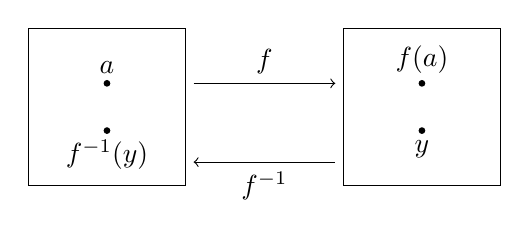
\begin{tikzpicture}

                  \draw[] (0,0) rectangle (2,2);
                  \draw[->] (2.1, 1.3) -- (3.9, 1.3) node[above, midway] {$f$};
                  \draw[<-] (2.1, 0.3) -- (3.9, 0.3) node[below, midway] {$f^{-1}$};

                  \draw[] (4,0) rectangle (6,2);


                  \filldraw[black] (1,1.3) circle (1pt) node[anchor=south]{$a$};
                  \filldraw[black] (5,1.3) circle (1pt) node[anchor=south]{$f(a)$};
                  \filldraw[black] (1,0.7) circle (1pt) node[anchor=north]{$f^{-1}(y)$};
                  \filldraw[black] (5,0.7) circle (1pt) node[anchor=north]{$y$};

              \end{tikzpicture}
          \end{center}
          Recall that $f \circ f^{-1} = I$, so differentiating and applying the chain rule we can write
          \begin{equation}
              f'(f^{-1}(y)) \cdot (f^{-1})'(y) = I \implies (f^{-1})'(y) = [f'(f^{-1}(y))]^{-1}
          \end{equation}
    \item We are allowed to write $f'(a) = I$ since every invertible matrix is just the identity with a change of basis. More concretely, consider another composition represented below, where $L=f'(a):$
          \begin{center}
              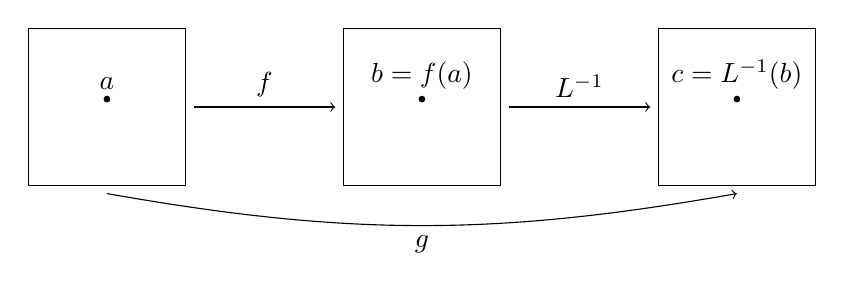
\begin{tikzpicture}

                  \draw[] (0,0) rectangle (2,2);
                  \draw[->] (2.1, 1) -- (3.9, 1) node[above, midway] {$f$};
                  \draw[->] (6.1, 1) -- (7.9, 1) node[above, midway] {$L^{-1}$};

                  \draw[] (4,0) rectangle (6,2);
                  \draw[] (8,0) rectangle (10,2);


                  \filldraw[black] (1,1.1) circle (1pt) node[anchor=south]{$a$};
                  \filldraw[black] (5,1.1) circle (1pt) node[anchor=south]{$b=f(a)$};
                  \filldraw[black] (9,1.1) circle (1pt) node[anchor=south]{$c=L^{-1}(b)$};

                  \draw [->,black] (1,-0.1) to [out=-10,in=190] node[below, midway] {$g$} (9,-0.1);

              \end{tikzpicture}
          \end{center}
          By the chain rule, we have $g'(a) = L^{-1} \circ f'(a)$ since $L^{-1}$ is a linear transformation. Note that $f'(a) = L$, so $g'(a) = I$ is the identity.

          If the IFT was true for functions whose differential is $I$, then it's true for $g$, so there exists $g^{-1}$. Also, $f^{-1} = g^{-1} \circ L^{-1}.$ Therefore, if $g^{-1}$ is continuously differentiable, then $f^{-1}$ would also be continuously differentiable. Thus, it is sufficient to only look at the case where the differential is the identity.

    \item Consider a small neighbourhood around $a$. Intuitively, we should expect vectors and the image of the vectors (which need not start at $a$) to look roughly the same.

          Specifically, $f$ has \textbf{all-scale-fidelity} on some neighbourhood $U$ of $a$ with \textit{fidelity factor} $\frac{1}{257}.$ This means for all $x_1,x_2 \in U$, we have
          \begin{equation}
              |(x_2-x_1) - (f(x_2)-f(x_1))| \le \frac{1}{257}|x_2-x_1|
          \end{equation}
          \begin{proof}
              From a previous theorem, if we have a function $g:\mathbb{R}^n\rightarrow\mathbb{R}^n$ whose derivative $|g'| < M$ is bounded in some open set, then we can write
              \begin{equation}
                  |g(x_1)-g(x_2)| < n^2M|x_1-x_2|.
              \end{equation}
              Now consider $g(x) = f(x) - x$. The derivative is $g'=f'-I$ so $g'(a)=0.$ Therefore, there exists an open rectangle $U$ of $a$ where we can say $|g'(x)| \le \frac{1}{257n^2}.$

              By the previous theorem, for any $x_1,x_2 \in U$, we have
              \begin{equation}
                  |g(x_1)-g(x_2)| \le \frac{1}{257}|x_1-x_2|
              \end{equation}
              However, the LHS is just
              \begin{align*}
                  |g(x_1)-g(x_2)| & = |f(x_1)-x_1-(f(x_2)-x_2)|   \\
                                  & = |(x_2-x_1)-(f(x_2)-f(x_1))|
              \end{align*}
          \end{proof}
    \item Given $y\in W$, we wish to find an $x \in V$ such that $f(x)=y$. We will travel this direction in $W$, but we may ``miss'' by a bit. We can then repeat this process, with each step we travel in the direction of $y$.

          Put this formally, let $W=B_{r/2}(b).$ Given $y\in W$, we claim that there exists an $x\in B_r(a)$ such that $f(x)=y.$ Indeed,
          \begin{align}
              x_1 & = a+(y-b)                  \\
              x_2 & = x_1+(y-f(x_1))           \\
              x_3 & = x_2+(y-f(x_2))           \\
              x_n & = x_{n-1} + (y-f(x_{n-1}))
          \end{align}
          But the difference between any two consecutive terms is just the LHS of the all-scale fidelity
          \begin{align}
              |x_n-x_{n-1}| & = |(x_{n-1}-x_{n-2})-(f(x_{n-1}-f(x_{n-2}))| \\
                            & \le \frac{1}{257}|x_{n-1}-x_{n-2}|           \\
                            & \le \frac{1}{257^{n-1}} |x_1-x_0|            \\
                            & \le \frac{1}{257^{n-1}} | y-b|               \\
                            & \le \frac{1}{257^{n-1}} \frac{r}{2}
          \end{align}
          We now need to show that each $x_i$ is within the ball of radius $r$ around $a$ (since this is only when all-scale fidelity is defined). It can be shown via induction that $|x_n-a| \le r.$

          Finally, we show that $(x_n)$ is a Cauchy-Sequence. We can immediately show this by noting that
          \begin{equation}
              |x_n-x_m| \le \frac{1}{257^m}r
          \end{equation}
          so $(x_n)$ is cauchy.
    \item While we have shown that $f(x_n)$ converges to $y$, we have not yet shown that this is possible, i.e. what if there is a discontinuity? We can invoke the continuity of $f$ to show that there does exist such an $x_n.$ We have
          \begin{equation}
              |f(x_n)-y| = |x_{n+1}-x_n| \le \frac{1}{257^n}\frac{r}{2} \rightarrow 0
          \end{equation}
          so from continuity, there exists an $x$ such that
          \begin{equation}
              |f(x)-y| = \lim_{n\to \infty} |f(x_n)-y|  = 0.
          \end{equation}
          Therefore, $f(x)=y.$ We can now define $V=F^{-1}(W)$ and now
          \begin{equation}
              F|_V: V\rightarrow W
          \end{equation}
          is onto and 1-1.
    \item We have constructed $x$ in one such way. How do we know that if we use a different procedure, we find a different $x$?

          Assume that $f(x_1)=f(x_2)$ where $x_{1,2} \in B_r(a).$ Then by ASF,
          \begin{align}
              |(x_1-x_2)-(f(x_1)-f(x_2))| & \le \frac{1}{257}|x_1-x_2| \\
              |x_1-x_2|                   & \le \frac{1}{257}|x_1-x_2|
          \end{align}
          which is true if and only if $x_1=x_2.$

    \item It might seem that continuity for $f^{-1}$ is cheap. After all, the difference between two vectors in both the input and image space is roughly the same. However, the mistake is written in terms of $|x_1-x_2|$, so this reasoning becomes circular. We need to reformulate the ASF principle such that the mistake is in terms of $|y_1-y_2|.$

          To simplify things, let $\alpha=x_1-x_2$ and $\beta=f(x_1)-f(x_2).$ Then ASF says that
          \begin{equation}
              |\alpha-\beta | \le \frac{1}{257}|\alpha|
          \end{equation}
          But $\alpha = \beta + \alpha - \beta$. By the triangle inequality, this becomes
          \begin{align}
              |\alpha-\beta |               & \le \frac{1}{257}(|\beta|+|\alpha-\beta|) \\
              \frac{256}{257}|\alpha-\beta| & \le \frac{1}{257}|\beta                   \\
              |\alpha-\beta|                & \le \frac{1}{256}\beta
          \end{align}

    \item Let us first show that $f^{-1}$ is differentiable at the point $b$. We can write
          \begin{equation}
              f^{-1}(b+h) = f^{-1}(b) + I\cdot h + e(h)
          \end{equation}
          We want to show that $e(h)$ is tiny. We want to rearrange this in a form such that we can apply all scale fidelity. Let $b+h = y_2$ and let $x_2=f^{-1}(y_2).$ Let $b=y_1$ and $a=x_1$, so the above just becomes
          \begin{equation}
              x_2 = x_1 + y_2-y_1 + e(h)
          \end{equation}
          However the error once rearranged becomes
          \begin{equation}
              |e(h)| = |(x_2-x_1)-(y_2-y_1)| \le \frac{1}{256}|y_2-y_1|
          \end{equation}
          Since $y_2-y_1=h$, we end up with
          \begin{equation}
              \frac{|e(h)|}{|h|} \le \frac{1}{256}
          \end{equation}
          Now we have a problem: we want to show that this approaches zero. This condition is not good enough. However, this constant was chosen arbitrarily, so we can make $\frac{|e(h)|}{|h|}$ as small as possible.
    \item Similarly, the choice of $b$ was also arbitrary. If the conditions for the IFT hold at $a$, then they have to hold in an open set near $a$ (due to continuity). Therefore, we can rewrite the entire proof by considering points near $b$ and not just $b$.
    \item To show $f^{-1}$ is continuously differentiable, we can use the chain rule:
          \begin{equation}
              (f^{-1})'(y) = [f'(f^{-1}(y))]^{-1}
          \end{equation}
          We can conclude that $f^{-1}(y)$ is continuous in $y$ and $f'(x)$ is continuous in $x$. Therefore, $M \mapsto M^{-1}$ is a continuous operation on matrices. Specifically, it is a function that maps $\mathbb{R}^{n^2}\rightarrow \mathbb{R}^{n^2}.$ This is not everywhere defined. But where defined, the inverse is continuous by Cramer's Law. There is an explicit formula for the inverse, so this map is continuous.
\end{enumerate}
\subsection{Implicit Function Theorem}
TBA

\newpage
\section{Integration}
\subsection{Rigorous Definition}
\subsubsection{Partitions}
Let $R = \prod_{i=1}^n\left([a_i,b_i]\right)$ be a rectangle in $\mathbb{R}^n$ and let $f:R\to\mathbb{R}$ be bounded. We lay out some definitions:
\begin{itemize}
    \item A \emf{partition} $P$ of $R$ is a sequence $(P_i)^n_{i=1},$ where $P_i$ is a partition of $[a_i,b_i]$ (i.e. $P=a_i=t_{i_0}\le t_{i_1}\le \cdots \le t_{i_{N_i}}=b_i$)
    \item When a \emf{sub-rectangle} $S$ is relative to partition $P$, we use the notation $S \in P$. If we choose integers $1\le j_i \le N_i$ for $i\in \{1,\dots,n\}$ and $j=(j_1,\dots,j_n),$ then it can be written as $S_j = \prod_{i=1}^n([t_{i,j_{i-1}},t_{i,j_i}])$.
    \item The volume of a rectangle is
    \begin{equation}
        \text{vol}(R) = |R| = \prod_{i=1}^n(b_i-a_i)
    \end{equation}
\end{itemize}
\subsubsection{Lower and Upper Sums}
Let $f:R\to \mathbb{R}$ be founded. Then
\begin{align}
    L(f,P) &= \text{lower sum of F rel P} = \sum_{S \in P}(\text{vol}(S) m_s(f)) \\ 
    U(f,P) &= \text{upper sum of F rel P} = \sum_{S \in P}(\text{vol}(S) M_s(f))
\end{align}
where $m_s \le M_s \implies L(f,P) \le U(f,P)$. A function is \emf{integrable} if $L(f,P)$ and $U(f,P)$ converge to each other.
\begin{proposition}
    If $P$ is a partition of $R$, then
    \begin{equation}
        \sum_{S\in P}(V(S)) = V(R)
    \end{equation}
\end{proposition}
\subsubsection{Refinements and Integrability Theorems}
\begin{definition}
    We say that $P'$ \emf{refines} $P$ if every $S'\in P'$ is a subset of some $S\in P$. Equivalently, if $S\in P \implies S = U_{S'\in P', s'\in S}(s')$.
\end{definition}
\begin{lemma}
    If a partition $P'$ refines a partition $P$, then
    \begin{align}
        L(f,P) &\le L(f,P') \\ 
        U(f,P) &\ge U(f,P')
    \end{align}
\end{lemma}
A direct corollary is that if $P_1,P_2$ are partitions of $R$ then $L(f,P_1) \le U(f,P_2).$
\begin{definition}
    \emf{Upper integral} of $f$ is
    \begin{equation}
        \text{inf}\{U(f,P)\} =: U(f) = \int_U f \\ 
    \end{equation}
    and the \emf{lower integral} of $f$ is
    \begin{equation}
        \text{sup}\{L(f,P)\} =: L(f) = \int_L f \\
    \end{equation}
\end{definition}
An alternative but equivalent way to say $f$ is \emf{integrable} is when $L(f)=U(f).$
\begin{theorem}
    The function $f$ is integrable if and only if for all $\epsilon >0$, there exists $P$ such that $U(f,P)-L(f,P) <\epsilon.$
\end{theorem}
\begin{theorem}
    Continuous functions are integrable.
\end{theorem}
\subsection{Measure Theory}
\begin{definition}
    $A$ is of \emf{measure-$0$} means that for $\forall \epsilon > 0$, there exists open (alternatively closed) rectangles $(R_i)_{i=1}^\infty$ such that
    \begin{enumerate}
        \item $A \subset \bigcup R_i$
        \item $\sum \text{vol}(R_i) < \epsilon.$
    \end{enumerate}
    Note that when we say measure 0, we refer to \emf{Lebesgue measure-$0$.}
\end{definition}
For example, finite \& countable sets, along with $\mathbb{R} \subset \mathbb{R}^2$ are of measure $0$.
\begin{definition}
    A set $X$ is called \emf{countably infinite} if there is a surjective function $F$ such that $F: \mathbb{N} \onto X$
\end{definition}
A few facts that follows:
\begin{enumerate}
    \item Finite sets are countable. (Typically, we exclude this from the definition.)
    \item Subsets of countable sets are countable. (Proof: Elements in a countable set can be enumerated. Simply select a new enumeration.)
    \item A finite/countable union of countable sets is countable. If $A_i$ is countable for all $i$, then $\bigcup A_i$ is countable.
          \begin{proof}
              Consider
              \begin{align*}
                  A_1: & \quad a_{11}\quad a_{12}\quad a_{13}\quad \cdots \\
                  A_2: & \quad a_{21}\quad a_{22}\quad a_{23}\quad \cdots \\
                  A_3: & \quad a_{31}\quad a_{32}\quad a_{33}\quad \cdots \\
              \end{align*}
              To enumerate the union, we look at the diagonals, i.e.
              \begin{equation}
                  \bigcup A = \{a_{11}, a_{12}, a_{21}, a_{13}, a_{22}, a_{31}, \dots \}
              \end{equation}
          \end{proof}
          Another fact that immediately follows is that the set of integers is countable, since $\mathbb{Z} = (-\mathbb{N})\cup \{0\} \cup \mathbb{N}$
    \item If $A,B$ are countable, then $A\times B$ is countable.
          \begin{proof}
              We can prove this similar to how a countable union of sets is countable. Alternatively, we can write
              \begin{equation}
                  A\times B = \bigcup_{b\in B} A \times \{b\}
              \end{equation}
              And each set $A\times \{b\}$ is coutnable.
          \end{proof}
          A fact that follows is that the set of rationals is countable, since $\mathbb{Q} \subset \mathbb{Z}\times \mathbb{Z}.$
\end{enumerate}
It may seem a bit suspicious since up to this point, everything is countable. However, there are sets that are uncountable!
\begin{theorem}
    $\mathbb{R}$ is not countable. And hence, irrational numbers are not countable, i.e. there are ``more'' reals than naturals, more irrationals than rationals.
\end{theorem}
\begin{proof}
    Assume that $\mathbb{R}$ is countable, that is $(a_i)$ is an enumeration of the real numbers. Let $x$ be a real number whose $k^\text{th}$ decimal digit is different from the $k^\text{th}$ decimal digit of $a_k$. Note that $x$ cannot be any of the $a_k$s, hence $\{a_k\}\neq \mathbb{R}$.
\end{proof}
We can now state and prove a few statements about measure-$0$.
\begin{enumerate}
    \item If $A$ is measure-$0$ and $B\subset A$, then $B$ is measure-$0$.
    \item A countable union of measure-$0$ sets is measure-$0$.
          \begin{proof}
              Suppose $\forall i$, $A_i$ is of measure $0$, so given $\epsilon > 0$, we can cover $A_i$ with countably many rectangles whose $\sum\text{vols} < \frac{\epsilon}{2^i}$. Take all the rectangles above together, as a countable collection of countable sets, this collection of rectangles is countable, and
              \begin{equation}
                  \sum\text{vols} < \sum_{i=1}^\infty \frac{\epsilon}{2^i} = \epsilon.
              \end{equation}
              Finally this collection covers
              \begin{equation}
                  \bigcup A_i = A
              \end{equation}
              so $A$ is measure-$0$.
          \end{proof}
          Note that we have stated before that $\mathbb{R} \subset \mathbb{R}^2$
\end{enumerate}
\begin{warning}
    Countable sets are measure-$0$, but the converse is not true! For example, $\mathbb{R}\subset\mathbb{R}^2$ has measure-$0$, but is not countable.
\end{warning}
Another Example: Let $\mathcal{C}$ be the \emf{cantor set} $\subset [0,1]$ which is uncountable, yet of measure-$0$ in $\mathbb{R}$. Let
\begin{equation}
    \mathcal{C} = \{0.C_1C_2C_3C_4\dots: C_i \in \{0,2\}\}
\end{equation}
$C$ is uncountable for the same reason as $\mathbb{R}$. Define $C_k$ to be the union of $2^k$ intervals of length $\frac{1}{3^k}$. Therefore,
\begin{equation}
    C \subset C_k
\end{equation}
where $C_k$ itself is a union of intervals of total length $2^k \cdot \frac{1}{3^k} = \left(\frac{2}{3}\right)^k$, which approaches $0$.

Therefore, $C$ is measure-$0$. As an aside, each $C_k$ is compact, so $\mathcal{C} = \cap C_K$ is therefore also compact.
\begin{theorem}
    $[a,b] \subset \mathbb{R}$ is \textit{not} measure $0$. In fact, $R \subset \mathbb{R}^n$ is not measure $0$.
\end{theorem}
\begin{definition}
    $A\subset \mathbb{R}^n$ is said to be of \emf{content-$0$} if $\forall \epsilon > 0$ it is contained in a finite union of rectangles whose sum of volumes is smaller than $\epsilon$.
\end{definition}
Note that $\mathbb{Z} \in \mathbb{R}$ is not of content-$0$. Note that content-$0$ refers to \emf{Jordan Measure $0$.}

A set is \emf{Jordan Measurable} (alternatively \emf{rectifiable}) as follows:
\begin{definition}
    $S$ is Jordan measurable if and only if $S$ is bounded and the boundary has measure $0$. 
\end{definition}
\begin{definition}
    $S$ is Jordan measurable if and only if the identity function is integrable over $S$.
\end{definition}
We can relate integrability and measure theory.
\begin{theorem}
    A function $f$ is integrable if and only if it is continuous except on a set of measure $0$.
\end{theorem}
\section{Fubini's Theorem}
Currently, we have the tools to define the integral, but we don't have the tools to compute the integral yet. We will start off with a loose example.
\begin{example}
    Integrate $xy$ on $[0,1]_x \times [0,1]_y.$ Fubini's theorem loosely tells us that we can fix $x$, and then fix $y$. Namely,
    \begin{equation}
        \int\limits_{[0,1]\times [0,1]}xy \dd{x}\dd{y} = \int_0^1 x \int_0^1 y \dd{y}\dd{x} = \frac{1}{4}
    \end{equation}
\end{example}
We will now formally state it.
\begin{theorem}
    \textbf{(Tempting but Incorrect)} Let $A\subset \mathbb{R}_x^n$ and $B\subset \mathbb{R}_y^m$ be rectangles, set $R=A\times B \subset \mathbb{R}^{n+m}.$ Let
    \begin{equation}
        F:R \rightarrow \mathbb{R}
    \end{equation}
    be an integrable function. Let
    \begin{equation}
        g(x) = \int\limits_{B} f(x,y) \dd{y}.
    \end{equation}
    Then
    \begin{equation}
        \int\limits_R F =  \int\limits_A g \dd{x}
    \end{equation}
    Note that this is incorrect for general functions $f$, but is true if $f$ is continuous.
\end{theorem}
\begin{warning}
    Note that we cannot define $g(x) = \int\limits_{B} f(x,y) \dd{y}$ and $\int\limits_A f = \int\limits_A g \dd{x}$ since while $f$ is integrable over $A\times B$, it is not necessarily integrable over $B$. For example, suppose we have a function defined as
    \begin{equation}
        f(x,y) = \begin{cases}
            0 & x < 0.5 \\
            1 & x > 0.5 \\
            1_{\mathbb{Q}}
        \end{cases}
    \end{equation}
    where $1_{\mathbb{Q}}$ is the Dirichlet function, defined to be $1$ if rational and $0$ otherwise. $f$ will be integrable in the region $[0,1]\times [0,1]$ but is not integrable if we restrict it to the line $x=0.5.$ This is because the set of discontinuities is of measure $0$ in $\mathbb{R}^2$ but is of measure $1$ in $\mathbb{R}$.
\end{warning}
While it may be tempting to write the theorem as
\begin{equation}
    g(x) = \begin{cases}
        \int\limits_B f(x,y) \dd{y} & \text{ f(x,-) is integrable} \\
        17                          & \text{ otherwise}.
    \end{cases}
\end{equation}
and define
\begin{equation}
    \int\limits_R f = \int\limits_A g
\end{equation}
which might solve the problem of discontinuities. However, this is still wrong. Here is a counter example.

Consider $h(x) = \begin{cases}
        \frac{1}{q} & x = \frac{p}{q}  \\
        0           & \text{otherwise}
    \end{cases}$ defined on $[0,1]$, known as Thomae's function, which looks like the below
\begin{center}
    % Draw Thomae's Function in Tikzpicture
    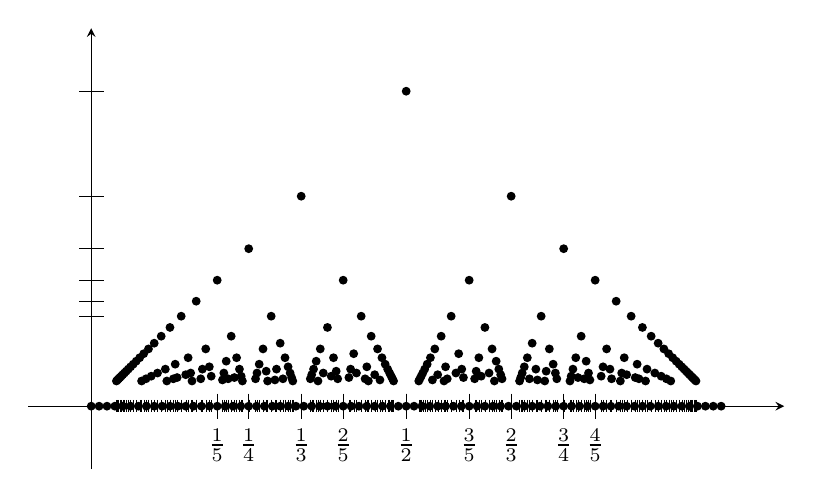
\begin{tikzpicture}[scale=8]
        \draw [-stealth] (-0.1,0) -- (1.1,0);
        \draw [-stealth] (0,-0.1) -- (0,0.6);
        \foreach \X in {1,...,7}
            {\ifnum\X=1
                \else
                    \draw (0.02,1/\X) -- (-0.02,1/\X) node[left,xshift={(-(1+pow(-1,\X)))*3pt}]{};
                \fi
            }
        \foreach \X [evaluate=\X as \Ymax using {int(\X-1)}]in {25,24,...,2}
        {\foreach \Y in {1,...,\Ymax}
            {\ifnum\X<6
                    \draw (\Y/\X,0.02) -- (\Y/\X,-0.02) node[below,fill=white]{$\frac{\Y}{\X}$};
                \else
                    \draw[ultra thin] (\Y/\X,0.01) -- (\Y/\X,-0.01);
                \fi
                \pgfmathtruncatemacro{\TST}{gcd(\X,\Y)}
                \ifnum\TST=1
                    \fill ({\Y/\X},1/\X) circle(0.2pt);
                \fi
            }
        }
        \foreach \X in {0,1,...,80}
            {\fill (\X/80,0) circle(0.2pt); }
    \end{tikzpicture}
\end{center}
Note that $h(x)$ is discontinuous on $\mathbb{Q}$ but continuous on $\mathbb{Q}^C$. Since $\mathbb{Q}$ is of measure $0$, $h$ is integrable. The integral is
\begin{equation}
    \int_0^1 h(x) = 0
\end{equation}
and we can prove this by cropping the function about some arbitrary $y=c.$ Since there are only a finite amount of points above this line, we can ``chop'' them off. Now we extend this to two variables. Consider
\begin{equation}
    f(x,y) = \begin{cases}
        \frac{1}{q} & x,y\in \mathbb{Q}, x=\frac{p}{q} \\
        0           & \text{otherwise}
    \end{cases}
\end{equation}
defined on the set $[0,1]\times [0,1]$. If we try to compute $g$ using the second incorrect attempt, we get
\begin{equation}
    g(x) = \begin{cases}
        0  & x \notin \mathbb{Q} \\
        17 & x \notin \mathbb{Q}
    \end{cases}
\end{equation}
but this is a ``bed of nails'' function with respect to $x$, and is not integrable, and thus we cannot expect an equality.

Note that the choice for $g(x)$ might sound stupid. After all, we can choose $0$ instead of $17$, to remove the problematic values. However, we can just shift $f(x,y)$ to create another counterexample.

Let us now state the correct theorem,
\begin{theorem}
    (Correct Fubini's Theorem) Let $A \subset \mathbb{R}_x^n$ and $B \subset \mathbb{R}_y^n$ be rectangles, set $R=A\times B \subset \mathbb{R}^{n+m}$. Let $f:R\rightarrow \mathbb{R}$ be an integrable function and let
    \begin{align}
        \ubar{g}(x) & = \int\limits_L f(x,y) \dd{y} = L(f(x,-)) = \sup \text{ lower sums for } f(x,-) \\
        \bar{g}(x)  & = \int\limits_U f(x,y) \dd{y} = U(f(x,-)) = \inf \text{ upper sums}
    \end{align}
    Then $\ubar{g}$ and $\bar{g}$ are integrable and
    \begin{equation}
        \int\limits_R f\dd{x}\dd{y} = \int\limits_A \ubar{g} \dd{x} = \int\limits_A \bar{g} \dd{x}
    \end{equation}
\end{theorem}
Let us go back to our previous counterexample. Now,
\begin{align}
    \ubar{g}(x) & = \begin{cases}
        0 & x\notin \mathbb{Q} \\
        0 & x\in \mathbb{Q}
    \end{cases}
\end{align}
so $\ubar{g}(x)=0$ and $\int \ubar{g} = \int 0 = 0.$ On the other hand,
\begin{equation}
    \bar{g}(x) = \begin{cases}
        0           & x\not\in Q \\
        \frac{1}{q} & x \in Q
    \end{cases}
\end{equation}
which is just $h(x)$ from earlier, which we have computed the integral already to be $0$. Now that we have worked through examples, but we have not yet proved the theorem yet.

Before we do so, note that if $f$ is continuous, all that is a non-issue
\begin{equation}
    g(x) = \int\limits_B f(x,y) \dd{y} = \bar{g}(x)=\ubar{g}(x)
\end{equation}
for all $x$, so the naive Fubini's Theorem holds. Likewise, if $f(x,-)$ is integrable except for finitely many $x$'s, then the second attempt we made holds.
\begin{proof}
    We sketch out the proof as follows:
    \begin{enumerate}
        \item Bound $L(f,P) \le L(\ubar{g},P_A)$ and $U(f,P) \le U(\bar{g}, P_A)$.
        \item Show that $\bar{g}$ and $\ubar{g}$ are integrable.
    \end{enumerate}
    We will now carry out these steps:
    \begin{enumerate}
        \item Consider a partition $P$ of $R \subset \mathbb{R}^{n+m},$ which is illustrated below. We can restrict our attention to the first $n$ and the last $m$ coordinates. We can always write it as $P_A \times P_B,$ where $P_A$ is a partition of $A$ and $P_B$ is a partition of $B$.
              \begin{center}
                  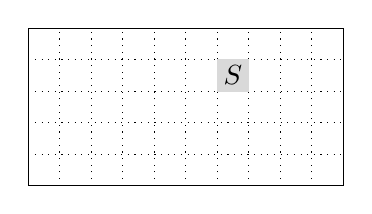
\begin{tikzpicture}
                      % Draw Rectangle
                      \draw (-2,-1) rectangle (2,1);
                      \foreach \x in {-2,-1.6,...,2}
                          {
                              \draw[dotted] (\x,-1) -- (\x,1);
                          }
                      \foreach \y in {-1,-0.6,...,1}
                          {
                              \draw[dotted] (-2,\y) -- (2,\y);
                          }
                      \filldraw[gray!30] (0.4,0.2) rectangle (0.8,0.6);
                      \node (S) at (0.6,0.4) {$S$};
                      % Node at (1.6, 0.4)

                  \end{tikzpicture}
              \end{center}
              If $S\in P$, we can write $S = S'\times S''$ where $S' \in P_A$ and $S'' \in P_B$.

              Given this partition $P=P_A \times P_B$ of $R$, we have
              \begin{align}
                  L(f,P) & = \sum_{S\in P} V(S) \cdot \inf\limits_{(x,y)\in S} f(x,y)                                               \\
                         & = \sum_{\substack{S'\in P_A                                                                              \\ S'' \in P_B}} V(S')V(S'') \cdot \inf\limits_{x \in S'} \inf\limits_{y \in S''} f(x,y)\\
                         & = \sum_{S' \in P_A}V(S') \sum_{S'' \in P_B} V(S'') \inf\limits_{x \in S'} \inf\limits_{y \in S''} f(x,y)
              \end{align}
              We are aiming to pull the infimums outside. We can do this with the following lemma.
              \begin{lemma}
                  Let $h_k: X\rightarrow \mathbb{R}_1$. Then
                  \begin{equation}
                      \sum_k \inf h_k(x) \le \inf \sum_k h_k(x)
                  \end{equation}
              \end{lemma}
              \begin{proof}
                  Note that $\inf\limits_x h_k(x) \le h_k(y)$ for all $y$ given any $k$. This means that we can sum both sides
                  \begin{equation}
                      \sum_k \inf h_k(x) \le \sum_k h_k(y)
                  \end{equation}
                  The left hand side is a constant but the right hand side is a function of $y$. Since this inequality is true for all $y$, we can just pick the $y$ to minimize the right hand side:
                  \begin{equation}
                      \sum_k \inf\limits_x h_k(x) \le \inf\limits_y \sum_y h_k(y)
                  \end{equation}
                  which is just the lemma with different variable names.
              \end{proof}
              Using this lemma, we can bound $L(f,P)$ by
              \begin{align}
                  L(f,P) & \le \sum_{S' \in P_A}V(S')\inf_{x\in S'}\underbrace{\sum_{S''\in P_B}V(S'')\inf_{y\in S''}f(x,y)}_{L(f(x,-),P_B)} \\
                         & \le \sum_{S' \in P_A}V(S')\inf\limits_{x\in S'}\ubar{g}(x)                                                        \\
                         & = L(\ubar{g},P_A)
              \end{align}
              Similarly, we can do the same thing with supremums to get
              \begin{equation}
                  L(f,P) \le L(\ubar{g}, P_A) \quad\quad\quad U(\bar{g}, P_A) \le U(f,P)
              \end{equation}
              \item Note that both $L(\bar{g},P_A)$ and $U(\ubar{g},P_A)$ are bounded by both $L(\ubar{g},P_A)$ (on the lower end) and $U(\bar{g},P_A)$ (on the upper end). Let us restrict our attention to
              \begin{equation}
                  L(\ubar{g}, P_A) \le U(\ubar{g}, P_A).
              \end{equation}
              This means that $\ubar{g}$ is integrable. Similarly, $\bar{g}$ is integrable.

              Now assume $\epsilon > 0$ and $P$ was chosen such that $U(f,P)-L(f,P) < \epsilon$ (which is possible since $f$ is integrable), then
              \begin{equation}
                  U(\ubar{g}, P_A) - L(\ubar{g}, P_A) \le \epsilon
              \end{equation}
              and 
              \begin{equation}
                    U(\bar{g}, P_A) - L(\bar{g}, P_A) \le \epsilon
              \end{equation}
              so $\ubar{g}$ and $\bar{g}$ are integrable on $A$.
              \item From the inequalities earlier, we can write  
              \begin{equation}
                  L(f,P) \le \int_A \bar{g}, \int_A \ubar{g} \le U(f,P)
              \end{equation}
              which is true for every $P$. This means that we can take the infimum and supremum over all partitions, to get
              \begin{equation}
                  \int f \le \int \bar{g}, \int \ubar{g} \le \int f
              \end{equation}
              so $\int f = \int \bar{g} = \int \ubar{g}$ and we are done.
    \end{enumerate}
\end{proof}
It turns out that we can ignore the upper and lower bound conditions if we have that $f_x(y)$ is integrable for all $x$, where $f_x(y)$ is $f$ restricted to a given $x$.

\newpage
\section{Partitions of Unity}
\subsection{Motivation}
We will answer the question of how we can integrate over a non-compact set. Similar issues appear in other areas: We know how things work on a small scale. How do we make it work on a large scale?

For example, we could say that to integrate over an unbounded set, we can partition the set by an infinite amount of intersecting rectangles, integrate over the rectangles, and then sum the integrals. However, this is not so easy to do.

Consider the example of two players trying to divide the work over two regions.
\begin{center}
    \begin{tikzpicture}
        \draw [] (-2, -2) -- (0.5, -2) -- (0.5, 2) -- (-2, 2);
        \draw [] (2, -2.1) -- (-0.5, -2.1) -- (-0.5, 2.1) -- (2, 2.1);

        \node (A) at (-2, 0) {$1$};
        \node (A') at (-2, -0.5) {$\phi_1$};
        \node (B) at (2, 0) {$2$};
        \node (A') at (2, -0.5) {$\phi_2$};
    \end{tikzpicture}
\end{center}
where $\phi_i$ represents the amount of work each player does. In each non-intersecting section, we want $\phi_i=1$ and in the shared section, we want to break up the work in some continuous fashion (i.e. close to player 1, player 1 does more work.)

Let us look at the general case where we want to divide up the work $W= \bigcup U_i$ across $n$ players. We can define $\phi_i$ on three conditions:
\begin{enumerate}
    \item The function $\phi_i$ is defined 
    \begin{equation}
        \phi_i: W \rightarrow [0,1]
    \end{equation}
    and we can let it be $C^\infty$. It turns out this condition can be weaker, but this stronger condition works out fine at the end. We also have the condition for all $x$,
    \begin{equation}
        \sum \phi_i(x) = 1
    \end{equation}
    \item We also want the support of the function to be a subset of $U_i$, that is $\supp \phi_i \subset U_i$, where the support of a function is defined as follows:
    \begin{equation}
        \supp \phi_i = \cl \{x:\phi_i(x) \neq 0\}
    \end{equation}
    \item We also want \textit{local finiteness}, where ever $x\in W$ has a neighbourhood $V \ni x$ such that 
    \begin{equation}
        \left|\{i: V \cap \supp \phi_i \} \right| < \infty.
    \end{equation}
\end{enumerate}
This is essentially what partitions of unity is about. We want to partition unity via functions $\phi_i(x).$ Our goal at the end is to show that if we have a function $f$ defined on a set $W \subset \bigcup U_i.$ 
\begin{equation}
    \int\limits_W f := \sum_i \int\limits_{U_i}\phi_i f
\end{equation}
\subsection{Theorem}
We propose the following theorem, which states that all of the above can be achieved:
\begin{theorem}
    Given $A\subset \mathbb{R}^n$ and given an open cover of $A$ defined as $\cal{U} = \{U_\alpha\}$ where $U_\alpha$ is open and $\bigcup_\alpha U_\alpha \supset A$, we can find a countable collection 
    \begin{equation}
        \Phi = \{\phi_i: W\rightarrow [0,1]\}
    \end{equation}
    of $C^\infty$ functions defined on some open set $W \supset A$ (where $W$ is defined to be slightly bigger than $A$) such that three conditions hold:
    \begin{enumerate}
        \item \textbf{Local Finiteness:} Every $x\in W$ has an open neighbourhood $V\ni x$ such that 
        \begin{equation}
            \left|\{i: V\cap \supp \phi_i \neq \emptyset\} \right| < \infty.
        \end{equation}
        \item \textbf{Sum is Unity:} For all $x\in A$, we have
        \begin{equation}
            \sum_{i=1}^\infty \phi_i(x) = 1
        \end{equation}
        Note that by the first condition, there are only a finite number of $\phi_i$ that is nonzero for each $i$, i.e. it is a ``nearly finite sum.''
        \item \textbf{Subordinate:} We have $\Phi$ is subordinate to $\cal{U}$, i.e. for all $i$, there exists an (not necessarily unique) $\alpha$ such that
        \begin{equation}
            \supp \phi_i \subset U_\alpha
        \end{equation}
        Note that this third condition is slightly different from the one in the motivation. This is because we can have an infinite cover. All this is insisting is that each ``worker'' has a set in which it does work.
    \end{enumerate}
\end{theorem}
\subsection{Proof}
We start with some preliminary lemmas.
\subsubsection{Preliminary 1: Finding a Smooth Bump}
We want to eventually find a function $\phi$ such that if we have a set $C\in U$, we want to find a function that is $1$ inside $C$ and $0$ outside $C$.
\begin{lemma}
    Given a compact $C$ contained in an open $U$, where $C \subset U$, there exists a $C^\infty$ function $\psi: U \rightarrow [0,1]$ such that 
    \begin{enumerate}
        \item $\psi|_C = 1$
        \item $\supp \psi \subset U$.
    \end{enumerate}
\end{lemma}
That is, if $\psi$ existed, then it could look like the following mountain (where the flat part is $C$, slanted part is $U$, and the rest is outside of $U$) 
\begin{center}
    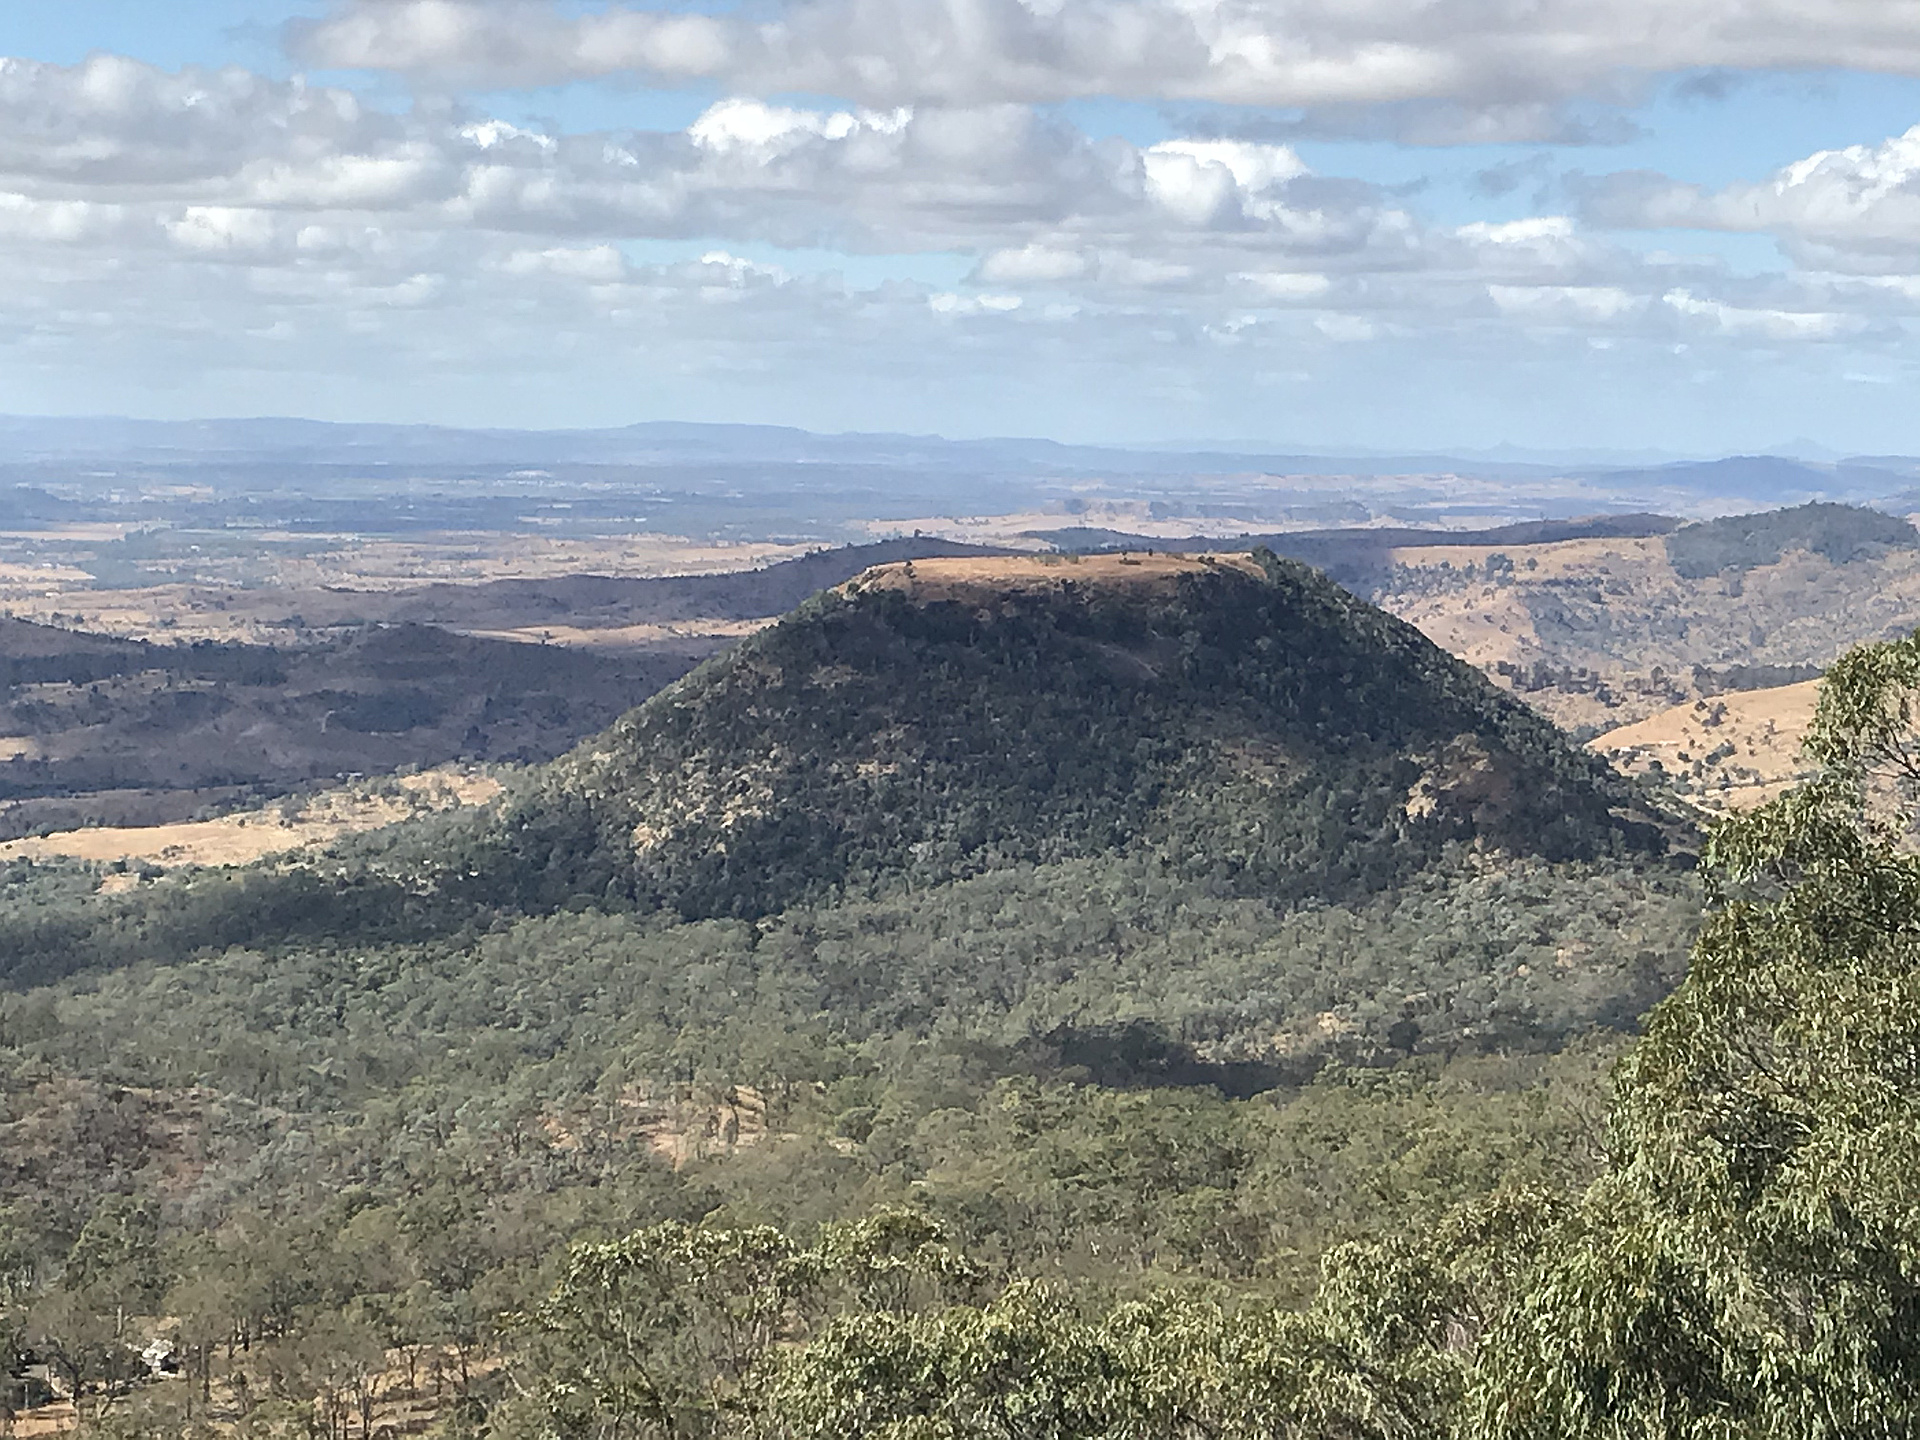
\includegraphics[width=0.5\linewidth]{figures/tabletop.jpg}
\end{center}
We should find proving this problematic since even in the simplest case, we don't know any functions that do this! However, we can still prove this.
\begin{proof}
    We take the following steps:
    \begin{enumerate}
        \item We restrict our attention to one dimension (i.e. a seashore). There exists a function $\sigma: \mathbb{R} \rightarrow \mathbb{R}$ such that 
        \begin{equation}
            \begin{cases}
                \sigma(x) = 0 & x \le 0 \\ 
                \sigma(x) > 0 & x > 0
            \end{cases}
        \end{equation}
        where $\sigma \in C^\infty$.
        \item There exists a smooth one-dimensional function $\beta_\epsilon$ that represents a bump such that
        \begin{equation}
            \begin{cases}
                \beta_\epsilon(x) = 0 & |x| > \epsilon \\ 
                \beta_\epsilon(0) > 0
            \end{cases}
        \end{equation} 
        \item We now look at the general case of $\mathbb{R}^n$. We wish to show that there exists an $n$-dimensional bump. Given $a \in \mathbb{R}^n$ and $\epsilon > 0$, there exists $\beta_{a,\epsilon}$ such that $\beta \in C^\infty$ and 
        \begin{equation}
            \begin{cases}
                \beta(a) > 0 & |x-a| < \epsilon \\
                \beta(x) = 0 & |x-a| \ge \epsilon
            \end{cases}
        \end{equation}
        \item Let's look at $\mathbb{R}$ again. There exists a smooth \textit{step} function $\sigma\in C^\infty$ and $\theta:\mathbb{R} \rightarrow [0,1]$ such that 
        \begin{equation}
            \begin{cases}
                \theta(x) = 0 & x \le 0 \\ 
                \theta(x) = 1 & x \ge 1
            \end{cases}
        \end{equation}
        \item We can construct a \textit{flaptop} mountain such that for some $C \subset U$, we have $f(x)=1$ and outside $U$ we have $f(x)=0.$
    \end{enumerate}
    Let us take these steps and prove them: 
    \begin{enumerate}
        \item In particular, we claim that \begin{equation}
            \sigma(x) = \begin{cases}
                e^{-1/x} & x > 0 \\ 
                0 & x \le 0
            \end{cases}
        \end{equation}
        is such a function.
        \begin{center}
            \begin{tikzpicture}
                \begin{axis}[
                legend pos=outer north east,
                title=Seashore Function,
                axis lines = middle,
                xlabel = $x$,
                ylabel = $y$,
                variable = t,
                trig format plots = rad,
                ymin = -1,
                ymax = 1,
                ]
                \addplot [
                    domain=0:1,
                    samples=400,
                    color=blue,
                    ]
                    {exp(-1/x)};
                \addplot [
                    domain=-1:0,
                    samples=70,
                    color=blue,
                    ]
                    {0};
                \end{axis}                
            \end{tikzpicture}
        \end{center}
        We can show $\sigma$ is smooth via the following: for $x>0$, we have
        \begin{align}
            \sigma' &= \frac{1}{x^2}e^{-1/x} \\ 
            \sigma'' &= \left(-\frac{2}{x^3}+\frac{1}{x^4}\right)e^{-1/x} \\ 
            \sigma^{(n)} &= r(x)e^{-1/x}
        \end{align}
        where $r(x)$ is some rational function, which we can prove via induction. We can also show that $\lim_{x\to 0} \sigma^{(n)} = 0$ since exponentials beat polynomials (it is not hard to show this formally). This is the key point to showing that the $n^\text{th}$ derivative approaches $0$ at $x=0$, and that $\sigma(x)$ is $C^\infty.$
        \item We can construct such a $\beta(x)$ by multiplying two seashore functions together. Namely,
        \begin{equation}
            \beta_\epsilon(x) =  \sigma(x+\epsilon)\sigma(\epsilon-x).
        \end{equation}
        To show this has the desired properties, we just need to apply the properties of $\sigma$.
        \item We can define 
        \begin{equation}
            \beta_{a,\epsilon}(x) := \beta_{\epsilon^2}(|x-a|^2)
        \end{equation}
        Since both $\beta_{\epsilon^2}$ and $|x-a|^2$ is smooth, this function is also smooth. Note that we couldn't have $|x-a|$ in the parameter since we want the function to be smooth, and we only know that the composition of two smooth function is smooth.
        \item Let us define
        \begin{equation}
            \theta_0(x) = \int_0^x \beta_{1/2,1/2}(t) \dd{t}
        \end{equation}
        and let 
        \begin{equation}
            \theta(x) = \frac{1}{\theta_0(1)}\theta_0(x)
        \end{equation}
        \item We can create a finite open cover for $C$. To show this, for each $x\in C$, we can find $\epsilon_x > 0$ such that $B_{\epsilon_x}(x) \subset U$ which is possible since $U$ is open. Then,
        \begin{equation}
            \{B_{\epsilon_x}(x)\}
        \end{equation}
        is an open cover of $C$, hence it has a finite subcover $x_i$ with $i=1,\dots, m $ and 
        \begin{equation}
            \bigcup_{i=1}^m B_{\epsilon_{x_i}}(x_i) \supset C.
        \end{equation}
        Our first guess for such a flaptop mountain function may be 
        \begin{equation}
            f_0(x) = \sum_{i=1}^m \beta_{x_i,\epsilon_{x_i}}(x)
        \end{equation}
        But we still need to crop this! Note that $f_0$ is a continuous function on a compact set bounded below by some $b > 0$ on $C$. The function we want is 
        \begin{equation}
            f(x) = \theta\left(\frac{1}{b}f_0(x)\right)
        \end{equation}
        
    \end{enumerate}
\end{proof}
\subsubsection{Preliminary 2: Separating a Compact Set Contained in Open Set}
Intuitively, a compact set contains its boundary while an open set is fuzzy around its boundary. Therefore, we should expect a gap between a compact set $C$ and an open set $U$.
\begin{lemma}
    Given a compact $C$ and an open $U$, where $C \subset U \subset \mathbb{R}^n$, there exists a compact $D$ such that 
    \begin{equation}
        C \subset \Int D \subset D \subset U
    \end{equation}
\end{lemma}
This lemma is a bit stronger than our intuition. It says that a compact set $C$ can be contained in an open set $\Int D$, which is contained in a compact set $D$ and is contained in an open set $U$.
\begin{proof}
    The lemma is intuitive: We can construct a finite open cover of $C$ contained in $U$, since $C$ is compact. We can then ``shrink'' each ball by a tiny bit and take the closure, so we can also find a finite closed cover of $C$. Taking the union, we have constructed such a $D$.

    Let's make this more rigorous. For each $x\in C$, we can find an open ball $B_x$ such that $\overline{B_x}\subset U.$  Clearly, $\{B_x\}_{x\in C}$ covers $C$. By compactness, it has a finite subcover $B_{x_i}$ where $i=1,\dots, p.$ Take 
    \begin{equation}
        D = \bigcup \overline{B_{x_i}},
    \end{equation}
    which is a finite union of closed and bounded sets, so $D$ is closed and bounded, hence it is compact. It is also easy to check that 
    \begin{equation}
        \Int D = \bigcup B_{x_i} \supset C.
    \end{equation}
\end{proof}
\subsubsection{Putting it All Together}
We can now put it all together and prove the Partition of Unity theorem, but we will separate it into cases.

\textbf{Case I: $A$ is compact:}

We can visualize this case: 
\begin{center}
    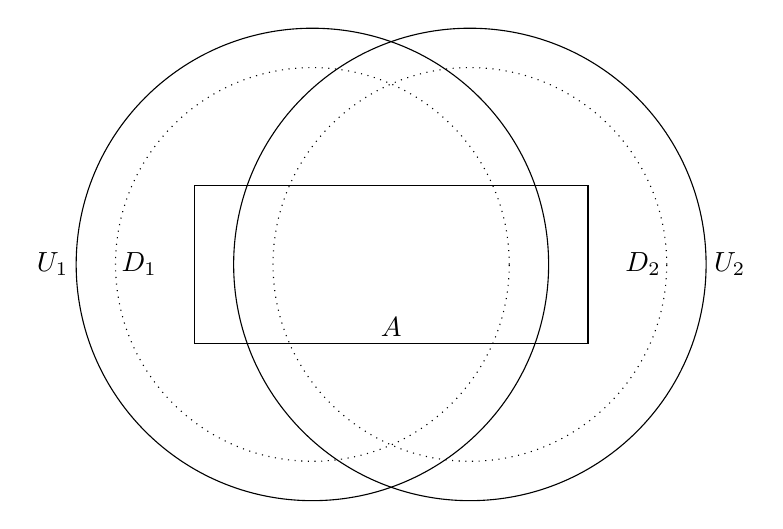
\begin{tikzpicture}
        
        \draw[] (-1,0) circle (3);
        \draw[] (1,0) circle (3);

        \draw[dotted] (-1,0) circle (2.5);
        \draw[dotted] (1,0) circle (2.5);


        \draw[] (-2.5,1) rectangle (2.5,-1);

        \node  at (-4.3,0) {$U_1$};
        \node  at (-3.2,0) {$D_1$};
        \node  at (4.3,0) {$U_2$};
        \node  at (3.2,0) {$D_2$};
        \node  at (0,-0.8) {$A$};

    \end{tikzpicture}
\end{center}
Since $A$ is compact, we can construct a finite open cover of $A$, i.e. $U_1 \subset U_2$, then by lemma 2, construct $D_1 \subset D_2$ to also be a cover. Intuitively, we want each worker to do some work inside $D_1$ but no work outside $U_1.$
\begin{proof}
    We perform the following steps: 
    \begin{enumerate}
        \item Define the exclusive zone of $U_1$ to be $E_1 = A \setminus \bigcup_{j=2}^p U_j$ and show that we can construct it.
        \item Show that we can ``Shrink'' each $U_i$ to a compact set $D_i$ such that $\{\Int D_i\}$ still covers $A$. Namely, we can find compact $D_i$ such that $D_i \subset U_i$ and $\bigcup \Int D_i \supset A.$
        \item Given the claim, we can find $\Psi_i:\mathbb{R}^n \to [0,1]$ which are $C^\infty$ such that $\Psi_i|_{D_i} \equiv 1$ and $\supp \Psi_i \subset U_i$. The $\Psi_i$ does not have to be $C^\infty$ at this point.
        \item Make the $\Psi_i$ a $C^\infty$ function by using preliminary 1.
    \end{enumerate}
    Let us now prove these statements.
    \begin{enumerate}
        \item Let $E_1$ denote the exclusive zone of $U_1$, and is equal to $E_1 = A \setminus \bigcup_{j=2}^p U_j.$ We know $E_1$ is compact and $E_1 \subset U_1.$
        
        By preliminary 2, we can find a compact set $D_1$ such that 
        \begin{equation}
            E_1 \subset \Int D_1 \subset D_1 \subset U_1.
        \end{equation}
        \item Let the \emf{exclusivity zone} for $U_1$ be $E_1$, defined as
        \begin{equation}
            E_1 = A \setminus \bigcup_{i=2}^{p}(U_i) \subseteq U_1.
        \end{equation}
        By preliminary 2, we can find a compact $D_1$ such that $E_1 \subseteq \text{int}(D_1) \subseteq D_1 \subseteq U_1$. Therefore, we have that
        \begin{equation}
            \text{int}(D_1) \cup \bigcup_{i=2}^pU_i \supseteq A.
        \end{equation}
        Suppose $D_1,\dots,D_{q-1}$ where $2\le q \le p$ have been constructed such that $D_i \subseteq U_i$ and \begin{equation}
            \bigcup_{i=1}^{q-1}(\text{int} D_i) \cup \bigcup_{i=q}^p(U_i) \supset A.
        \end{equation}
        In words, this says that we can ``shrink'' some $U_i$ to $\text{int} D_i$, and when joined with the other $U_i$, it still forms a cover for $A$. Let us set 
        \begin{equation}
            E_q = A \setminus \left(\bigcup_{i=1}^{q-1}\text{int}(D_i) \bigcup_{i=q+1}^p U_i\right).
        \end{equation}
        Then $E_q$ is compact, $E_q \subseteq U_q$, so we can use preliminary 2 to find $D_q$ such that $E_q \subset \text{int}(D_q) \subseteq D_q \subseteq U_q$. This is true for $q=2$, and we can repeat until $q=p$.
        \item We can define 
        \begin{equation}
            \psi_i(x) = \begin{cases}
                \frac{\Psi_i(x)}{\sum_{j=1}^{p} \Psi_j(x)} & x \in \bigcup \Int D_i \supset A \\ 
                0 & x \notin \bigcup \Int D_i
            \end{cases}
        \end{equation}
        Note that the denominator cannot be zero when $x\in \bigcup \Int D_i \supset A$, since it will contain all the $\Psi_i |_{D_i}$. However, we might have continuity issues on the boundary of $\bigcup \Int D_i,$ since it may be zero right outside and nonzero directly inside.
        \item We can multiply by a function $f(x)$ such that 
        \begin{equation}
            \psi_i(x) = \begin{cases}
                f(x) \frac{\Psi_i(x)}{\sum_{j=1}^{p} \Psi_j(x)} & x \in \bigcup \Int D_i \supset A \\ 
                0 & x \notin \bigcup \Int D_i
            \end{cases}
        \end{equation} 
        where $f(x)$ is smooth and satisfies $f|_A \equiv 1$ and $\supp f \subset \bigcup \Int D_i.$ We can construct an even smaller cover $\mathcal{V}$ than $\bigcup D_i$ such that outside, $f(x) = 0$ and inside $\mathcal{V}$, we have $f(x)=1.$ This ensures that $\psi_i$ is smooth.
    \end{enumerate}
\end{proof}
\textbf{Case II: $A$ is in the form of $A = \bigcup_{k=0}^{\infty} A_k$ where $A_k$ is compact and $A_k \subseteq \text{int}(A_{k+1})$:} Let us define
\begin{equation}
    L_k = A_{k+1} - \text{int}(A_k)
\end{equation}
for $k \ge 0.$ Let
\begin{equation}
    \mathcal{U}_k = \{U \cap \text{int}(A_{k+2}) \cap A_{k-1}^C | U \in \mathcal{U}\}.
\end{equation}
Note that since the interior is open, $U_k$ is open. We can use step 1 to find a partition of unity $\psi_k = \{\psi_{k_i}\}$ for $L_k$ and subordinate to $U_k$. Let
\begin{equation}
    \Psi = \bigcup_{k=0}^{\infty} \psi_k = \{\psi_i\},
\end{equation}
which is a countable collection of $C^\infty$ functions. We can set 
\begin{equation}
    \phi_i(x) = \frac{\psi_i(x)}{\sum_{j=1}^{\infty} \psi_j(x)}.
\end{equation}
Clearly, $\{\phi_i\}$ is the desired partition of unity for $A = \bigcup(A_k).$

\textbf{Case III: $A$ is an arbitrary open set:} Let us write 
\begin{equation}
    A = \bigcup_{k \ge 1}(A_k)
\end{equation}
where 
\begin{equation}
    A_k = \left\{x\in A: |x| \le k \text{ and } \text{dist}(x,A^c) \le \frac{1}{k}\right\}.
\end{equation}
Our claim is then $A_k$ is contained in $\text{int}(A_{k+1}).$ Each $A_k$ is compact, and $\bigcup_{k \ge 1}(A_k) = A.$ Therefore, by case II, we are done.
\section{Integration on Unbounded Sets}
We have only defined integration of bounded functions on bounded sets. We can extend this to unbounded functions on unbounded sets. We wish to define a new integration denoted by $NT$ (for new technology) and relate it to the legacy definition of integration.

Our goal is to show that 
\begin{equation}
    \int^{NT}\limits_A F = \sum_{i} \int \phi_i f.
\end{equation}
where $NT$ stands for new technology, which will allow us to integrate over unbounded sets.

We start off with a few preliminaries that worked for our legacy definition of integration.
\begin{enumerate}
    \item Assuming $f$ and $g$ are integrable, we have 
    \begin{align}
        \int\limits_{R} (f+g) &= \int\limits_{R} f + \int\limits_{R} g 
    \end{align}
    \item If $c$ is a scalar, we have
    \begin{equation}
        \int\limits_{R} cf = c\int\limits_{R} f
    \end{equation}
\end{enumerate}
\begin{warning}
    However, be warned that things become super wack for infinite sums. The \textbf{Riemann Rearrangement Theorem} tells us that we can re-arrange these sums to get any sum you want. The reason is as follows: Suppose we have the sum 
\begin{equation}
    1-\frac{1}{2}+\frac{1}{3}-\frac{1}{4}+\frac{1}{5}+\cdots,
\end{equation}
we can divide it into two groups:
\begin{equation}
    1,\frac{1}{3},\frac{1}{5},\frac{1}{7}, \dots \quad\quad\quad\quad\quad\quad -\frac{1}{2}, -\frac{1}{4}, -\frac{1}{6}, -\frac{1}{8},\dots
\end{equation}
Note that both the left and right group diverges. I can set this sum equal to $257$ by permuting the terms such that we first construct a number slightly above $257$ using the left terms, then subtract some right terms to get slightly below $257$, and since we have an infinite amount of numbers on both sides, we can have it bounce back and forth and eventually converge to $257$. This sequence of steps is always possible if 
\begin{equation}
    \sum |a_n| = \infty
\end{equation}
and 
\begin{equation}
    \sum a_n \text{converges}
\end{equation}
Recall from 157 that $\sum a_i$ is absolutely convergent if $\sum |a_i| <\infty.$ If this is the case, then the above nonsense does not work. The commutative law for an infinite sum then holds.
\end{warning}
\subsection{Setup}
We want to use our legacy definition of integration on functions acting on unbounded sets. To save work, we want to be able to relate the two.

Let $A$ be an open set that is not necessarily bounded. Let $f$ be a function $f:A\rightarrow \mathbb{R}$ with the following properties:
\begin{enumerate}
    \item $f$ is \emf{locally bounded}
    \begin{definition}
        A set $A$ is locally bounded if for all $x\in A$, there exists an open $V \ni x$ such that $f$ is bounded on $V$.
    \end{definition}
    \item $f$ is continuous except on a measure-$0$ set.
\end{enumerate}
Let $U=\{\mathcal{U}\}$ be an open cover of $A$ by bounded sets on which $f$ is bounded. Then let $\Phi = \{\phi_i\}$ be a partition of unity for $A$ subordinate to $U$.

We wish to show that 
\begin{equation}
    \int^{NT}\limits_{A} f = \sum_i \int \phi_i f.
\end{equation}
Note that we didn't specify the region of integration of the right hand side, but this doesn't matter since $\Phi$ is subordinate to $\mathcal{U}$, so we can define the region of integration to a rectangle bigger than $\supp \phi_i.$ There are three problems with this that we can fix:
\begin{itemize}
    \item How do we know that $\int \phi_i f$ is integrable?
    \item How do we know that the infinite sum converges and doesn't do anything weird?
    \item How do we know that a different choice of $\mathcal{U}$ and a partition of unity doesn't affect this?
\end{itemize}
We fix this by saying that $f$ is $(U,\Phi)$-integrable if 
\begin{equation}
    \sum_i \int\phi_i |f| < \infty
\end{equation}
In that case, we define 
\begin{equation}
    \int\limits_A^{(U,\Phi)} f := \sum_{i} \int \phi_i f.
\end{equation}
We want to later show that this doesn't depend on $U$ and $\Phi.$ Note that this series is absolutely convergent since
\begin{equation}
    \sum \left|\int \phi_i f\right| \le \sum \int|\phi_i f| = \sum\int_{\infty}\phi_i |f| < \infty
\end{equation}
so the weird things with rearrangements do not occur; the sum becomes well behaved.
\subsection{Choice of PO1 and Open Cover are Irrelevant}
We wish to show that 
\begin{theorem}
    If $A$ and $f$ are as before, then
    \begin{enumerate}
        \item If $U,U'$ and $\Phi,\Phi'$ are open covers and partitions of unity as before, then: $f$ is $(U,\Phi)$-integrable if and only if $f$ is $(U',\Phi')$-integrable.
        \item If $f$ is integrable (NT), then
        \begin{equation}
            \int^{(U',\Phi')}\limits_{A} f = \int^{(U,\Phi)}\limits_{A} f.
        \end{equation}
        In that case,
        \begin{equation}
            \int^{NT}\limits_{A} f := \int^{(U',\Phi')}\limits_{A} f = \int^{(U,\Phi)}\limits_{A} f.
        \end{equation}
    \end{enumerate}
\end{theorem}
We will also show that this new definition of the integral is equivalent to the old definition, when we have bounded functions in bounded sets.
\begin{proof}
    We will write a chain of equalities:
    \begin{align}
        \int^{(U,\Phi)}\limits_{A} g &\eq_{(1)} \sum_{i}\int \phi_i g \\ 
        &\eq_{(2)} \sum_{i}\int \left(\sum_j \phi_j' \right)\phi_i g \\
        &\eq_{(3)} \sum_i \sum_j \int \phi_j'\phi_i g \\
        &\eq_{(4)} \sum_j \sum_i \int \phi_i\phi_j' g \\
        &\eq_{(3)} \sum_j \int \left(\sum_i \phi_i\right)\phi_j' g \\
        &\eq_{(2)} \sum_j \int \phi_j' g \\
        &\eq_{(1)} \int^{(U', \Phi')}\limits_{A} g
    \end{align}
    Let us go through the above first with $g=|f|$. For this pass, we just need to show that the sum at the top converges if and only if the sum at the bottom converges.
    \begin{enumerate}
        \item Irrelevant
        \item Sum is $1$ in a partition of unity
        \item Integration is linear, but we have to be a bit more careful when dealing with infinite sums. We need to show that
        \begin{equation}
            \int \left(\sum \phi_j'\right) h  = \sum \int \phi_j' h,
        \end{equation}
        where $\supp h \subset \supp \phi_i \subset U \in \mathcal{U},$ so $\supp h$ is bounded and closed, hence it is compact. Therefore, byu compactness of $\supp h$ and local finiteness of $\Phi_i'$, only finitely many $i$ satisfy
        \begin{equation}
            \supp \phi_i' \cap \supp h \neq \emptyset.
        \end{equation}
        Hence, this holds by finite linearity.
        \item Note that $\phi_i\phi_j' = \phi_j'\phi_i$ due to commutativity. Now, we need to show that we can switch the sums. We have $|g|, \phi_1 \ge 0, \phi_j' \ge 0$ so all terms of the sums are non-negative. By the following exercise, we're done.
        
        \textbf{Exercise:} A sum of non-negative terms is convergent if and only if every rearrangement thereof is convergent.
    \end{enumerate}

    We wish to repeat the above steps for $g=f$. We now work under the assumption that the function is integrable, so the sums are absolutely convergent. The first step is by definition, the next two steps are the same as above, and the last step is true by absolute convergence.
\end{proof}
\subsection{NT Agrees with Old for Bounded Sets and Functions}
We wish to show that NT and old integration is irrelevant when $A$ and $f$ are both bounded. However, the old integration might not even exist since we can write
\begin{equation}
    \int\limits_A^{\text{old}} f = \int\limits_{\text{big R}}^{\text{old}} \chi_A f
\end{equation} 
where $\chi$ is the characteristic function
\begin{equation}
    \chi_A = \begin{cases}
        1 & x\in A \\ 
        0 & x\notin A
    \end{cases}
\end{equation}
and we need to make sure $\chi_A$ is continuous except on a set of measure-$0$.
\begin{theorem}
    The following are true, keeping the same definitions as above:
    \begin{enumerate}
        \item If $A$ and $f$ are bounded, then $f$ is NT-integrable on $A$.
        \item If in addition $A$ is Jordan Measurable, then
        the new integration is equivalent to the old integration.
    \end{enumerate}
\end{theorem}
\begin{proof}
    We will prove both parts:
    \begin{enumerate}
        \item Assume $|f| < M$ and $A \subset R$ where $R$ is some rectangle. We need to consider
        \begin{equation}
            \sum \int \phi_i |f|
        \end{equation}
        If this is finite, then $f$ is NT-integrable. Let us write the following chain of equalities:
        \begin{equation}
            \sum \int_R \phi_i |f| = \int_R \sum \phi_i |f| = \int_R |f| \le \int_R M =  M\text{vol}(R).
        \end{equation}
        The only problem with this is interchanging the integral and summation symbol. However, this is a non-issue since we can restrict our attention to some finite subset of the $\phi_i$'s. For example, we can write the chain as 
        \begin{equation}
            \sum_{i=1}^N \int_R \phi_i |f| = \int_R \sum_{i}^N \phi_i |f| \le \int_R M =  M\text{vol}(R).
        \end{equation}
        An infinite sum is convergent if and only if all the partial sums converge, so we are done.
        \item To prove the second part, we need the following lemma.
        \begin{lemma}
            For all $\epsilon > 0$, we can find a compact Jordan-measurable set $C \subset A$ such that $\text{vol}(A-C) < \epsilon.$
        \end{lemma}
        The proof is given in A8Q1. Assuming lemma, for only finitely many $i$'s, $\text{supp}(\phi_i) \cap C = \emptyset.$ We can find an $N$ bigger than all of those $i$'s, such that $\sum_{i=1}^{N}(\phi_i) = 1$ on $C$. Let us write down the following sequence of equality and inequalities:
        \begin{align}
            \left|\int\limits_{A}^{\text{old}} f - \sum_{i=1}^N \int^{\text{old}}(\phi_i f)\right| &= \left|\int\limits_A \left(f - \sum_{i=1}^N \phi_i f\right)\right| \\
            &\le \int \left(|f| \cdot \left(1 - \sum_{i=1}^N \phi_i\right)\right) \\ 
            &\le M\int \left(1-\sum_{i=1}^N \phi_i\right) \\ 
            &\le M\int\limits_{A-C}(1) \\ 
            &\le M \cdot \text{vol}(A-C) \\ 
            &\le M\cdot \epsilon,
        \end{align}
        and we are done.
    \end{enumerate}
\end{proof}
We still have a few more things to show. Namely, NT integration is linear and applying Fubini to NT integration.
\subsection{Other Properties of NT Integration}
The proof that NT integration is linear. Assuming $f$ and $g$ are integrable, we need to show that $f+g$ is integrable. To do this, pick the same open cover and PO1. The integral in each open ball is the same as the old way of integrating. The sum of two absolutely converging series is absolutely converging, so we are done. Then,
\begin{equation}
    \int_A^{NT} (f+g) = \sum_{i=1}^{\infty} \int \phi_i(f+g) = \sum_{i=1}^{\infty} \left(\int \phi_i \cdot f + \int \phi_i \cdot g\right) = \int f + \int g.
\end{equation}
Finally, we will show that Fubini applies to NT-integration as well. If $A\subset \mathbb{R}^n$ and $B\subset \mathbb{R}^n$ are open, $f:A\times B \to \mathbb{R}$ is locally bounded and continuous, except for finitely many points. Then,
\begin{equation}
    \int\limits_{A\times B} (f(x,y)) \dd{x}\dd{y} = \int\limits_A \dd{x} \int\limits_B \dd{y} f(x,y),
\end{equation}
assuming $f$ is integrable on $A\times B$. If:
\begin{itemize}
    \item $\mathcal{U}$ is an open cover of $A$
    \item $\mathcal{V}$ is an open cover of $B$.
    \item $\Phi = \{\phi_i\}$
    \item $\Psi = \{\psi_i\}$
\end{itemize}
then let us take $\mathcal{W} = \{U\times V: U \in \mathcal{U},V\in\mathcal{V}\}$ is an open cover of $A\times B$ and $\Lambda = \{\lambda_{i,j}=\phi_i(x) \cdot \phi_j(x)\}$ is a partition of unity for $A\times B$ subordinate to $W$. Note that
\begin{equation}
    \sum_{i=1}^{\infty}(\lambda_{i,j}(x,y)) = \sum_{i,j}(\phi_i(x) \cdot \phi_j(y)) = 1\cdot 1 = 1.
\end{equation}
Once we have this, NT-fubini reduces to old-fubini.
\newpage
\section{Change of Variables}
\begin{theorem}
    Let $A\subset \mathbb{R}^n$ is open, and let $g: A\rightarrow \mathbb{R}^n$ is continuously differentiable, 1-1, and $\forall a\in A$, $g'(a)$ is invertible. If $f:g(A) \rightarrow \mathbb{R}$ is integrable, then
    \begin{equation}
        \int\limits_{g(A)} f = \int\limits_{A} (f \circ g) |\det g'|
    \end{equation}
\end{theorem}
This is a powerful theorem. We can use it to compute the \emf{Gaussian integral}, which people often refer to it as the most important integral in mathematics:
\begin{equation}
    \int_{-\infty}^{\infty} e^{-x^2/2} \dd{x} = \sqrt{2\pi}
\end{equation}
\begin{proof}
    Let us name $I_1 = \int\limits_{\mathbb{R}} e^{-x^2/2}.$ Instead of computing this, let us compute 
    \begin{equation}
        I_2 = \int\limits_{\mathbb{R}^2} e^{-(x^2+y^2)/2} \dd{x}\dd{y}.
    \end{equation}
    Then, since NT-integration is linear:
    \begin{align}
        \int\limits_{\mathbb{R}^2} e^{-(x^2+y^2)/2} \dd{x}\dd{y} &= \int\limits_{\mathbb{R}} \dd{x}\int\limits_{\mathbb{R}} e^{-(x^2+y^2)/2} \\ 
        &= \int\limits_{\mathbb{R}} \dd{x} e^{-(x^2)/2} \int\limits_{\mathbb{R}} e^{-(y^2)/2} \\
        &= I_1^2
    \end{align}
    Let us now compute $I_2$ by switching to polar coordinates. To do so, consider the map
    \begin{equation}
        g(r,\theta) = \begin{pmatrix}
            r\cos\theta \\ r\sin\theta.
        \end{pmatrix}
    \end{equation}
    Then,
    \begin{equation}
        \det g' = \det \begin{pmatrix}
            \cos\theta & -r\sin\theta \\ 
            \sin\theta & r\cos\theta.
        \end{pmatrix} = r.
    \end{equation}
    Therefore, applying the COV formula, we have
    \begin{align}
        \int\limits_{g(A)} f &= \int\limits_{A} (f \circ g) |\det g'| \\ 
        &= \int \dd{r}\dd{\theta}e^{-r^2/2} r \\ 
        &= 2\pi.
    \end{align}
    Therefore, $I_1=\sqrt{2\pi}.$
\end{proof}
However in the above proof, we ignored two things. First, we applied Fubini's on integrals with infinite bounds, and secondly we ignored the distinction between open and closed sets. That is, integrating over the following two sets is equivalent:
\begin{equation}
    [0,\infty) \times [0,2\pi] \leftrightarrow (0,\infty) \times (0,2\pi).
\end{equation}
Let us address these issues:
\begin{enumerate}
    \item We can rewrite
    \begin{equation}
        \int\limits_{\mathbb{R} \times \mathbb{R}} e^{-\frac{x^2+y^2}{2}} \dd{x} \dd{y} = \left(\int\limits_{\mathbb{R}} e^{-x^2/2}\dd{x}\right) \left(\int\limits_{\mathbb{R}} e^{-y^2/2}\dd{y}\right)
    \end{equation}
    as
    \begin{equation}
        a_N = \int\limits_{[-N,N]^2} e^{-\frac{x^2+y^2}{2}} \dd{x} \dd{y} = \left(\int\limits_{-N,N} e^{-x^2/2} \dd{x}\right)\left(\int\limits_{-N,N}e^{-y^2/2}\dd{y}\right),
    \end{equation}
    which is true via the old Fubini's Theorem. What remains to show is that as $N\to\infty$, all three integrals converge to each other. Intuitively, this makes sense since the function ``descends rapidly,'' but this is not formal.
    
    To be rigorous, define
    \begin{equation}
        \int f \equiv \int\limits_{\mathbb{R}\times\mathbb{R}} e^{-(x^2+y^2)/2} \ge 0
    \end{equation}
    which is equal to, according to POI:
    \begin{equation}
        \int f = \sum_{i=1}^\infty \phi_i f = \lim_{p\to\infty}\sum_{i}^p \int \phi_i f.
    \end{equation}
    Since the $\phi_i$ have finite support, so we can interchange the integral and summation:
    \begin{equation}
        \int f = \int \left(\sum_{i=1}^p \phi_i\right) f \equiv b_p. 
    \end{equation}
    We now want to show that $a_N$ and $b_P$ have the same limit. Note that both $a_N$ and $b_P$ are both increasing sequences. If we can show that for all $N$, there exists an $N$ such that $b_p \ge a_N$ and for all $p$, there exists $N$ such that $a_N \ge b_P$, then
    \begin{equation}
        \lim_{p\to\infty} b_p = \lim_{N\to\infty} a_N.
    \end{equation}
    To show that these two properties are true, we can do the following:
    \begin{itemize}
        \item To show that there exists a $P$, we can pick a $p$ such that $\sum_{i=1}^p \phi_i(x) = 1$ on $[-N,N]^2,$ which implies that 
        \begin{equation}
            \sum \phi_i \ge \chi_{[-N,N]^2}.
        \end{equation}
        Therefore:
        \begin{equation}
            b_p = \int \left(\sum_{i=1}^p \phi_i\right)f \ge \int \chi_{[-N,N]^2}f = a_N.
        \end{equation}
        \item The proof is exactly the same. For large enough $N$, the square $[-N,N]^2$ contains the support,
        \begin{equation}
            [-N,N]^2 \supset \supp\sum_{i=1}^p \phi_i
        \end{equation}
    \end{itemize}
    \item The general idea is that you can always ignore closed sets of measure-$0$. This is because compact sets of measure-$0$ are content-$0$ and thus can be ignored.
    \begin{warning}
        This is not the case with ignoring general sets. If we change the value of a function on a set of measure-$0$, then we can introduce a lot of issues (i.e. continuity). However, if the set of measure-$0$ is also closed, we do not have any issues.
    \end{warning}
\end{enumerate}
\subsection{Layer Preserving Map}
\begin{definition}
    A function $g:\mathbb{R}\to\mathbb{R}^n$ is layer preserving if $g\left(x_1,\dots,x_n\right)=\left(\cdots,x_n\right).$ That is, the last coordinate stays the same.
\end{definition}
As an analogy, consider Prof. Dror's stacked books. We can integrate by going one layer at a time and then integrating over the book. We hope this will reduce the COV formula for $g$ to the COV formula for $g$ restricted to a given layer. This suggests that we might be able to prove the COV formula for layer preserving maps using induction.
\subsection{Proof}
\begin{proof}
    We will do the following:
    \begin{enumerate}
        \item If the theorem holds for two functions, then it holds for the composition. 
        \item If the COV formula holds in dimensions $n-1$, that it applies in $n$ dimensions (for layer preserving maps).
        \item Show that $g$ can be written as a composition of linear preserving maps.
        \item If the COV formula holds for small sets, then it holds for large sets.
        \item COV holds for the identity.
        \item The restricted COV formula implies the general COV formula holds.
    \end{enumerate}
    And to prove the above:
    \begin{enumerate}
        \item Consider the following composition of functions:
        \begin{equation}
            A \xrightarrow[h]{} h(A) \xrightarrow[g]{} (g\circ h)(A) \xrightarrow[f]{} \mathbb{R}.
        \end{equation}
        Then by the COV formula for $g$, we can write:
        \begin{equation}
            \int\limits_{(g\circ h)(A)} f = \int\limits_{h(A)} (f\circ g)|\det g'|.
        \end{equation}
        Let us define $\bar{f} \equiv (f\circ g)|\det g'|$, and apply the COV formula for $h.$ We get:
        \begin{equation}
            \int\limits_{h(A)} \bar{f} = \int\limits_{A} (\bar{f}\circ h)|\det h'|.
        \end{equation}
        Substituting in $\bar{f}$ and using the chain law, we have what is desired.
        \item Assume that COV holds for $n-1$ dimensions. Let $g: U \rightarrow \mathbb{R}^n$ where $U$ is an open bounded set and let $g$ be a layer-preserving map such that $g(U)$ is bounded. We then want to show the following restricted formula for $\text{cov}(g)$ holds: namely if $f:g(U) \to \mathbb{R}$ is continuous and $\supp f \subset g(U)$, then
        \begin{equation}
            \int\limits_{g(U)} f = \int\limits_{U} (f\circ g)|\det g'|.
        \end{equation}
        We don't actually need to specify the domain of integration, since the support is contained in $g(U).$ For any $z\in\mathbb{R}$, define $g_Z:\mathbb{R}^{n-1}\rightarrow \mathbb{R}^{n-1}$ by 
        \begin{equation}
            g_z(x) = \begin{pmatrix}
                g_1(x,z) \\ \vdots \\ g_{n-1}(x,z)
            \end{pmatrix}
        \end{equation}
        and define $f_Z:\mathbb{R}^{n-1}\rightarrow \mathbb{R}$ by $f_z(x) = f(x,z)$. The integral is thus 
        \begin{equation}
            \int f = \int\limits_{\mathbb{R}} \dd{z} \int\limits_{\mathbb{R}^{n-1}} \dd{x} f(x,z) = \int\limits_{\mathbb{R}} \dd{z} \int\limits_{\mathbb{R}^{n-1}} f_z(x)
        \end{equation}
        Using our inductive hypothesis (COV holds for $n-1$ dimensions), we can rewrite the integral as 
        \begin{equation}
            \int\limits_{\mathbb{R}} \dd{z} \int\limits_{\mathbb{R}^{n-1}} (f_z(x) \circ g_z) \cdot |\det g_z'|.
        \end{equation}
        Recall the derivative is written as the Jacobian 
        \begin{equation}
            g' = \begin{pmatrix}
                \frac{\partial g_1}{\partial x_1} & \cdots & \frac{\partial g}{\partial x_{n-1}} & \frac{\partial g_1}{\partial z} \\ 
                \vdots & \ddots & \vdots & \vdots \\
                \frac{\partial g_{n-1}}{\partial x_1} & \cdots & \frac{\partial g_{n-1}}{\partial x_{n-1}} & \frac{\partial g_{n-1}}{\partial z} \\ 
                \frac{\partial g_n}{\partial x_1} & \cdots & \frac{\partial g_{n-1}}{\partial x_{n-1}} & 1
            \end{pmatrix}
        \end{equation}
        \item Let $g:\mathbb{R}^n_{x_1}\rightarrow \mathbb{R}^n_{y_1}$ be an arbitrary function such that it maps $(x_1,\dots,x_n)$ to $(y_1,\dots,y_n)$ via $y_i = g_i(x_1,\dots,x_n)$. We can break up this map in the following way:
         \begin{equation}
             \begin{pmatrix}
                 x_1 \\ \vdots \\ x_n
             \end{pmatrix}
            \xrightarrow[]{\alpha}
            \begin{pmatrix}
                x_1 \\ \vdots \\ x_{n-1} \\ y_n
            \end{pmatrix}
            \xrightarrow[]{\beta}
            \begin{pmatrix}
                y_1 \\ \vdots \\ y_{n}
            \end{pmatrix}
         \end{equation}
         Note that $\alpha$ and $\beta$ are invertible, which can be shown using the inverse function theorem.
    \end{enumerate}
\end{proof}
\subsection{Baby Sard's Theorem}
We will give a brief overview of Sard's Theorem, and revisit it with greater rigor when we discuss Stoke's Theorem. Suppose we want to map $\{(r,\theta): r \ge 0, 0 \le \theta \le 2\pi\}$ to $\mathbb{R}^2.$ Note that this does not meet the conditions for COV since $\{(0,\theta):0\le \theta\le 2\pi\}$ gets mapped to $(0,0)$, so this map is not injective. However, intuitively, it feels like we can still use the COV formula in this case. A corollary of Sard's Theorem makes this official.

Namely, we can drop the condition that $g'$ is $1-1.$
\begin{theorem}
    (Baby Sard Theorem) Suppose we have open $A \subset \mathbb{R}^n$ and $g:A\rightarrow \mathbb{R}^n$ is continuously differentiable. Define:
    \begin{equation}
        C = \text{``critical set of $g$''} = \{x\in A| \det g'(x) = 0\}.
    \end{equation}
    Then $g(C)$ is of measure-$0$.
\end{theorem}
The nomenclature comes from in 1-dimension, $C$ is literally the set of critical values, since $\det g'(x) = g'(x)$ in single-variable calculus. It is important to note that we take the image of $C$. For example, consider a smooth bump. Clearly, the set of $x$ values at which the slope is zero is not of measure-0, since it is a continuous range in $\mathbb{R}.$

\textbf{Claim:} $A \setminus C$ is closed.
\begin{proof}
    The function $h(x) \equiv \det g'(x)$ is continuous since $g$ is continuously differentiable and the determinant just involves combining terms in the matrix (which are continuous), so $h$ is continuous. Then:
    \begin{equation}
        C = h^{-1}\{0\}.
    \end{equation} 
    For continuous functions, the pre-image of a closed set is a closed set
\end{proof}

\textbf{Corollary:} In the COV theorem, we can drop the condition $g'$ is 1-1 (equivalently invertible).
\begin{proof}
    Suppose we map $A$ to $g(A).$ Define $C \in A$ to be the closed set where $g'(C)$ is not invertible. While $C$ may not be of measure-0, $g(C)$ is of measure-0.

    First, we show that $g(A)$ is closed. To do this, we can write $g(A) \setminus g(C) = g(A\setminus C).$ Note that $A\setminus C$ is an open set of which $g'$ is invertible. Therefore, the inverse function theorem applies, so $g(A\setminus C)$ is open.
    
    Then:
    \begin{equation}
        \int\limits_{g(A)} f = \int\limits_{g(A\setminus C)} f.
    \end{equation}
    and
    \begin{equation}
        \int\limits_{A}(f\circ g)|\det g'| = \int\limits_{A\setminus C}(f\circ g)|\det g'|.
    \end{equation}
    By the old COV theorem, the relevant conditions are satisfied for $\int\limits_{A\setminus C}(f\circ g)|\det g'| = \int\limits_{g(A\setminus C)} f$ and using the equalities above, we can show the new version of COV.
\end{proof}
We can give a \textit{baby} proof of baby Sard. We will not go into details, since this is only a sketch
\begin{enumerate}
    \item Restrict attention to $A$ is a rectangle, and there is some subset $C\in A$ such that $g'(C)$ is not invertible.
    \item Partition $A$ into several subrectangles. For the subrectangles that touch $C$, then there will be a point where $g'$ is not onto, i.e. it maps to a smaller dimensional subspace. This subrectangles will not be mapped into a $n-1$ dimensional subspace, but will be mapped to a neighbourhood of one.
    \item This shows that we can cover $g(C)$ with rectangles where one dimension is very, very narrow, so this suggests it is of measure-$0$. 
\end{enumerate}
\subsection{Adult Sard's Theorem}
We can generalize Sard's theorem to a map from $n$ dimensions to $m$ dimensions.
\begin{theorem}
    Let $A$ be an open set and $g:A\subset\mathbb{R}^n \rightarrow \mathbb{R}^m.$ Define 
    \begin{equation}
        C = \{x\in A| \text{rank}g' < m\},
    \end{equation}
    and $g$ is $k$ times continuously differentiable, where $k=\max(1,n-m+1).$ Then $g(C)$ is measure-0. 
\end{theorem}
This is a much harder theorem to prove!
\section{K-Vector}
\begin{definition}
    Let $V$ be a vector space over $\mathbb{R}$ and $k\in \mathbb{N} = \mathbb{Z}_{\ge 0}$. Then: $T:V^k \rightarrow \mathbb{R}$ is called \emf{multi-linear} or \emf{k-linear} if
    \begin{equation}
        T(u_1,\dots,\alpha u_1' + \beta u_1{''}, \dots, u_k) = \alpha T(u_1,\dots,u_1',\dots,u_k)+\beta T(u_1,\dots,u_1'',\dots,u_k).
    \end{equation}
\end{definition}
Let us look at some examples. An inner product is a 2-linear map $\langle u_1,u_2\rangle \in \mathbb{R}$. An example of a 1-linear map is a linear map $\phi:V\rightarrow \mathbb{R}$ where $\phi \in V^*.$ An example of an n-linear map is the determinant. An example of a 0-linear is $w:V^0 = \{()\} \rightarrow \mathbb{R}$. Note that $V^0$ has a single element.
\begin{definition}
    Define
    \begin{equation}
        \mathcal{T}^k(V) = \{\text{k-linear maps on V}\}.
    \end{equation}
    Note that many other sources call it $\mathcal{T}^k(V^*).$
\end{definition}
This means that $\langle,\rangle \in \mathcal{T}^2V$, $\det \in \mathcal{T}^nV$, $\mathcal{T}^0V \cong \mathbb{R}$, and $\mathcal{T}'V = V^*.$ The set $\mathcal{T}^k(V)$ is related to the things that we can integrate, so we will later think about the dimensions.

\textbf{Review:} Suppose $v_1,\dots,v_n$ is a basis of $V$. Then there exists a unique basis $\phi_1,\dots,\phi_n$ of $V^* = \mathcal{T}^1V$ such that
\begin{equation}
    \phi_i(v_j) = \delta_{ij} = \begin{cases}
        1 & i=j \\ 
        0 & \text{otherwise}.
    \end{cases}
\end{equation}
Then $\{\phi_i\}$ is called the \emf{the dual basis of $(v_1,\dots,v_n)$}.

Let us give some more examples. For example, what is the dual basis of $\left\{\begin{pmatrix}
    1 \\ 2
\end{pmatrix},\begin{pmatrix}
    3 \\ 4
\end{pmatrix}\right\}$? Recall that $\mathbb{R}^2$ can be thought of as the set of column vectors while $(\mathbb{R}^2)^*$ can be thought of as the set of row vectors. The properties that we want are:
\begin{align}
    \phi_1(v_1) = 1 &\quad\quad \phi_1(v_2) = 0 \\
    \phi_2(v_1) = 0 &\quad\quad \phi_2(v_2) = 1.
\end{align}
These set of equations are equivalent to
\begin{equation}
    \begin{pmatrix}
        \phi_1 \\ 
        \phi_2
    \end{pmatrix}
    \begin{pmatrix}
        v_1 & v_2
    \end{pmatrix}
    = \begin{pmatrix}
        1 & 0 \\
        0 & 1
    \end{pmatrix}.
\end{equation}
Therefore,
\begin{equation}
    \begin{pmatrix}
        \phi_1 \\ \phi_2
    \end{pmatrix} = \begin{pmatrix}
        v_1 & v_2
    \end{pmatrix}^{-1} = \begin{pmatrix}
        1 & 3 \\ 
        2 & 4
    \end{pmatrix}^{-1} = \begin{pmatrix}
        -2 & 3/2 \\ 
        1 & -1/2
    \end{pmatrix},
\end{equation}
so $\phi_1=(-2,3/2)$ and $\phi_2=(1,-1/2)$.

\textbf{Claim:} $\mathcal{T}^k(V)$ is itself a vector space.

\emf{Tensor multiplication} is denoted with the map $\otimes:\mathcal{T}^k \times \mathcal{T}^\ell \rightarrow \mathcal{T}^{k+\ell}$ defined by 
\begin{equation}
    (T_1 \otimes T_2)(u_1,\dots,u_{k+\ell}) = T_1(u_1,\dots,u_k)\cdots T_2(u_{k+1},\cdots,u_{k+\ell}).
\end{equation}
\textbf{Claim:} $\mathcal{T}_1\otimes \mathcal{T}_2 = \mathcal{T}_1\mathcal{T}_2 \in \mathcal{T}^{k+\ell}$.
\subsection{Properties and Notation}
Here are some properties of vectors
\begin{itemize}
    \item Associativity: $T_1(T_2T_3)=(T_1T_2)T_3$
    \item Distributivity: $(T_1+T_2)T_3 = T_1T_2+T_1T_3$ (More specifically, bilinear.)
\end{itemize}
Note that multiplication isn't necessarily commutative. Consider the counterexample $e_1,e_2 \in \mathbb{R}^2$ and $\phi_1,\phi_2\in \mathcal{T}'(V).$ Then:
\begin{align*}
    (\phi_1\phi_2)(e_1,e_2) = \phi_1(e_1)\phi_2(e_2) = 1 \cdot 1 = 1\\ 
    (\phi_2\phi_1)(e_1,e_2) = \phi_2(e_1)\phi_1(e_2) = 0 \cdot 0 = 0
\end{align*}
\begin{definition}
    Let $\underline{n} = \{1,\dots,n\}$. Then
    \begin{equation}
        \underline{n}^k = \{\bar{i} = I =(i_1,\dots,i_k):i_\alpha \in \underline{n}\}.
    \end{equation}
\end{definition}
This notation is nice since $|\underline{n}^k| = n^k$. Let $(v_j)^n_{j=1} \in V^n$ and $J \in n^k,$ where $J$ is known as a \emf{multi-index}. Let us write
\begin{equation}
    V_J = (V_{j_1},V_{j_2},\dots,V_{j_k}).
\end{equation}
Then $\phi_i \in V^*$ for $i=1,\dots,n$, $I \in \underline{n}^k$, and $\phi_I = \phi_{i_1}\cdot \cdots \cdot \phi_{i_k}.$
\begin{itemize}
    \item \textbf{Example:} Consider our previous counterexample. We can re-write it as
    \begin{align*}
        \phi_1\phi_2 - \phi_{(1,2)} &\quad\quad \phi_{(1,2)}(e_{(1,2)}) = 1 \\ 
        \phi_2\phi_1 = \phi_{(2,1)} &\quad\quad \phi_{(2,1)}(e_{(1,2)}) = 0
    \end{align*}
\end{itemize}
Suppose $V$ is a vector space with basis $v_1,\dots,v_n$ and dual basis $\phi_1,\dots,\phi_n,$ and $I,J \in \underline{n}^k.$ Then
\begin{align}
    \mathcal{T}^k &= \phi_I(v_J) \\ 
    &= (\phi_{i_1}\cdots \phi_{i_k})(V_{j_i}\cdots V_{j_k}) \\
    &= \prod_{\alpha=1}^k \phi_{i_\alpha}(V_{j_\alpha}) \\ 
    &= \prod_{\alpha=1}^k \delta_{i_\alpha j_\alpha} \\ 
    &= \begin{cases}
        1 & I=J \\ 
        0 & I \neq J
    \end{cases}
\end{align}
\subsection{Theorem}
We are finally ready for our first theorem!
\begin{theorem}
    Let $V$ be a vector space with respect to a basis $v_1,\dots,v_n$ and dual basis $\phi_1,\dots,\phi_n$. Then:
    \begin{equation}
        \{\phi_I:I\in \underline{n}^k\}
    \end{equation}
    is a basis of $\mathcal{T}^k(V),$ and hence, the dimension is
    \begin{equation}
        \dim \mathcal{T}^kV = n^k.
    \end{equation}
\end{theorem}
This allows us to better understand the space of $k$-tensors. We prove this step by step through a series of lemmas.
\begin{lemma}
    If $T_1,T_2\in\mathcal{T}^k$, then $T_1=T_2 \iff \forall I, T_1(V_I)=T_2(V_I)$.
\end{lemma}
\begin{proof}
    The forwards direction is obvious. To prove the backwards direction, assume that for all $I$, we have $T_1(V_I)=T_2(V_I)$. Then set $T=T_1-T_2$. Therefore:
    \begin{align*}
        T(u_1,\dots,u_k) = T\left(\sum_{{i_1}=1}^n a_{1,i_1}v_1,\sum a_{2,i_2}v_2,\dots,\sum a_{k,i_k}v_k\right),
    \end{align*}
    and applying linearity, we end up with
    \begin{align*}
        T(u_1,\dots,u_k) &= (\text{sum and product of coefficients})(T_1(V_I)-T_2(V_I)) = 0 \\ 
        &\implies T = 0 \implies T_1=T_2.
    \end{align*}
\end{proof}
\begin{lemma}
    The set $\{\phi_I\}$ spans $\mathcal{T}^kV.$
\end{lemma}
Let us verify that this lemma makes sense first. Given $T\in \mathcal{T}^k$, does it make sense that $T$ can be written as a linear combination of $\phi_I$, specifically $T\stackrel{?}{=} \sum_I a_I\phi_I.$ The trick is to evaluate both sides on $V_J$, to get
\begin{align*}
    T(V_J) &= \sum_I a_I\phi_I(V_J) \\ 
    &= \sum_{I} a_I\delta_{IJ} = a_J.
\end{align*}
Note that we found a formula for $a_J$, so we're nearly done! Let us turn this into a formal proof.
\begin{proof}
    Given $T\in \mathcal{T}^k$, set $a_I =  T(V_I)$, and then I claim that $T = \sum_I a_I\phi_I$. To check two tensors are equal to each other, we can use lemma 1. All we need to show is
    \begin{align*}
        T(V_J) &= \left(\sum a_I\phi_I\right)(V_J).
    \end{align*}
    But, by definition, $T(V_J)=a_J$ and the RHS is $a_J$ as well from the above discussion.
\end{proof}
\section{Tidbits}
\subsection{Volume of Spheres}
Let's compute like physicists! Let
\begin{equation}
    \sigma_n = \text{vol}(S^n),\quad\quad S^n = \{x \in \mathbb{R}^{n+1}: |x|=1\}
\end{equation}
Note that $S_1$ is just the unit circle, $S_2$ is the unit sphere, and $S_0$ is just two points. To do so, we compute $I_{n+1}$, which is the Gaussian integral in $n+1$ dimensions. We have 
\begin{equation}
    I_{n+1} = \int\limits_{\mathbb{R}^{n+1}} e^{-|z|^2/2} \dd{z} = \int\limits_{\mathbb{R}^{n+1}} e^{-(z_1^2+\cdots+z_{n+1}^2)/2}\dd{z}_1\cdots \dd{z}_{n+1} = I_1^{n+1} = \left(2\pi\right)^{(n+1)/2}
\end{equation}
Also note that $e^{-|z|^2/2}$ is constant on spheres. Therefore, 
\begin{equation}
    I_{n+1} = \int\limits_{\mathbb{R}^{n+1}}e^{-|z|^2/2}\dd{z} = \int_0^\infty \dd{r} \text{vol}(S^n_r)e^{-r^2/2} = \sigma_n \int r^n e^{-r^2/2} \dd{r}
\end{equation}
where we define $\sigma_n$ to be $\text{vol}(S^n)$. Note that $\text{vol}(S_r^n) = \text{vol}(rS_1^n)=r^n\text{vol}(S^n) = r^n \sigma_n.$ Therefore, we have:
\begin{equation}
    I_{n+1} = \sigma_n \iota_n = (2\pi)^{(n+1)/2}
\end{equation}
We don't know how to compute $\iota_n$, but we can still work with it. For example, 
\begin{align}
    \iota_{n-2} &= \int_0^\infty \underbrace{r^{n-2}}_{u'}\underbrace{e^{-r^2/2}}_{v}\dd{r} \\ 
    &= -\int_0^\infty \frac{1}{n-1}r^{n-1} \cdot \left(-re^{-r^2/2}\right) \dd{r}  + uv\Big|_0^\infty \\ 
    &= \frac{1}{n-1} \int_0^\infty r^n e^{-r^2/2}\dd{r} + 0 \\
    &= \frac{1}{n-1}\iota_n 
\end{align}
which is true for $n>1.$ Therefore, $\sigma_n$ is
\begin{equation}
    \sigma_n = \frac{(2\pi)^{(n+1)/2}}{\iota_n} = \frac{2\pi \cdot (2\pi)^{(n-1)/2}}{(n-1)\iota_{n-2}} = \frac{2\pi}{n-1}\sigma_n 
\end{equation}
where we have constructed a recurrence relation for $\sigma_n$. We have
\begin{align}
    \sigma_0 &= 2 \\ 
    \sigma_1 &= 2\pi \\ 
    \sigma_2 &= 4\pi \\
    \sigma_3 &= 2\pi^2.
\end{align}
Let $\beta_n = \text{vol}(B_1(0) \subset \mathbb{R}).$ Then we can compute
\begin{equation}
    \beta_n = \int_0^1 \sigma_nr^n \dd{r}.
\end{equation}
\end{document}